\documentclass[xcolor=dvipsnames,aspectratio=1610]{beamer}

\usepackage{graphicx}
\usepackage[scale=2]{ccicons}
\usepackage{multicol}
\usepackage{enumitem}
\usepackage{xcolor}
\usepackage[absolute,overlay]{textpos}
% \usepackage[texcoord,grid,gridunit=mm,gridcolor=red!10,subgridcolor=green!10]
% {eso-pic}

\setitemize{label=\usebeamerfont*{itemize item}%
  \usebeamercolor[fg]{itemize item}
  \usebeamertemplate{itemize item}}

\newcommand{\exampleheight}{1.9cm}
\newcommand{\examplewidth}{16cm}

\usetheme[numbering=counter, progressbar=frametitle, sectionpage=none]{metropolis}
\setbeamercolor{background canvas}{bg=white}


\title{Conflict-Free Vertex Coloring of Planar Graphs}
\date{April 15, 2017}
\author{Shawn Seymour}

\begin{document}
  \maketitle

  \begin{frame}
    \begin{figure}[h]
      \centering
      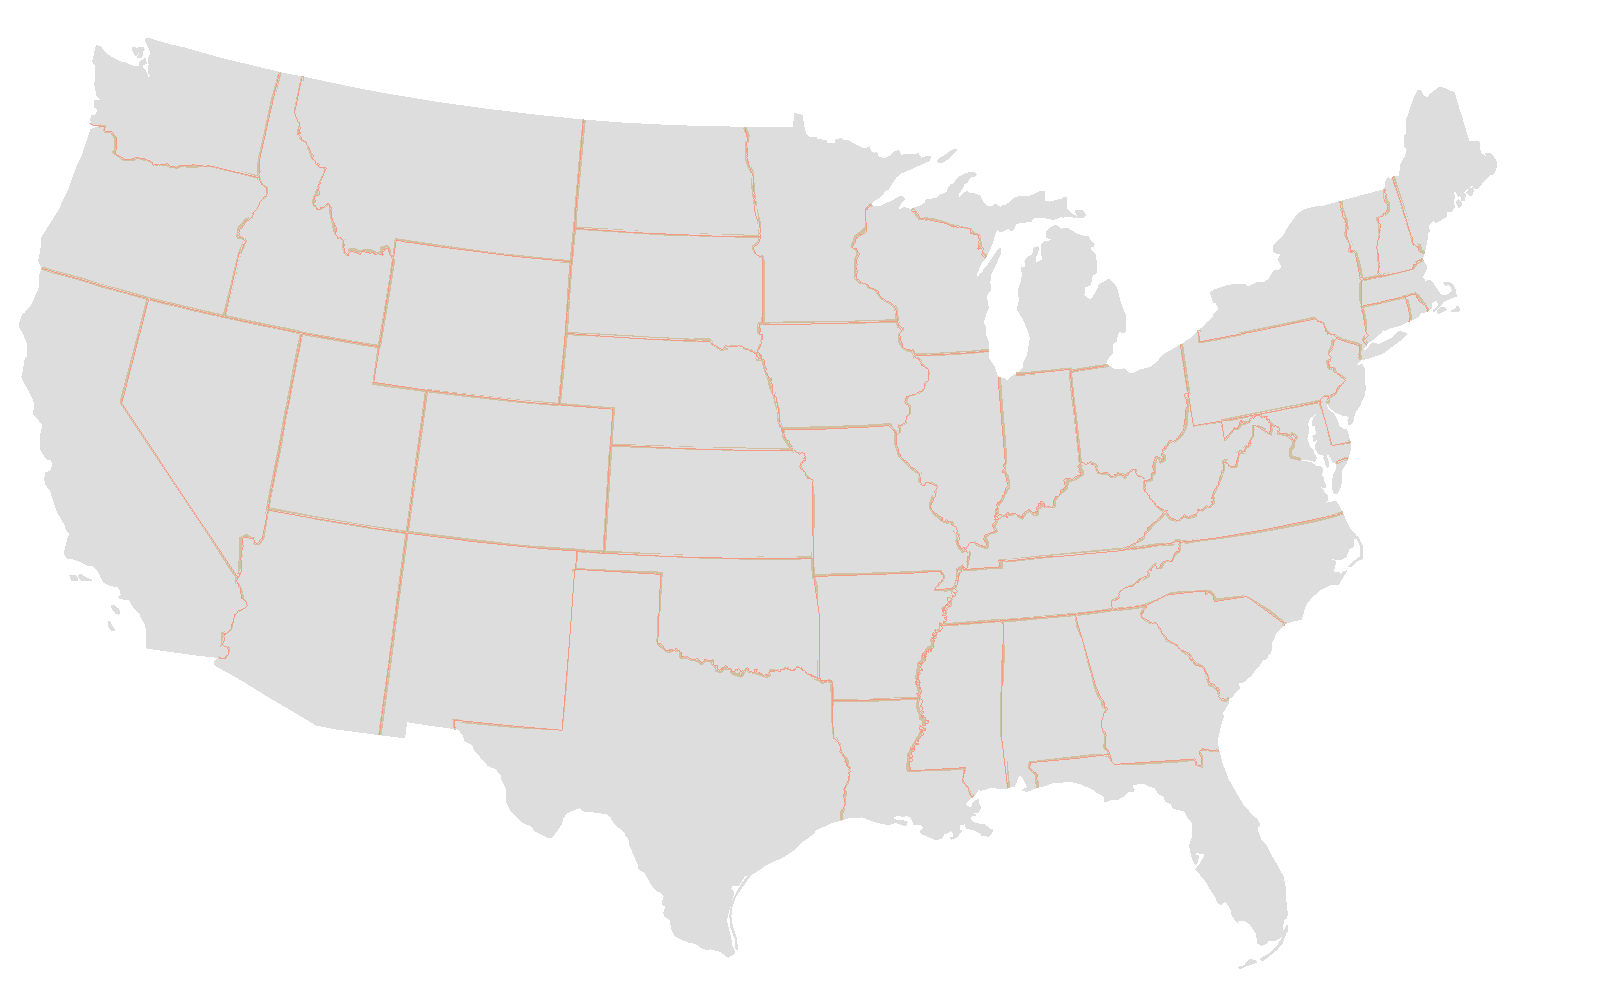
\includegraphics[width=14cm]{../figures/map-no-colors-3.pdf}
    \end{figure}
  \end{frame}

  \begin{frame}
    \begin{figure}[h]
      \centering
      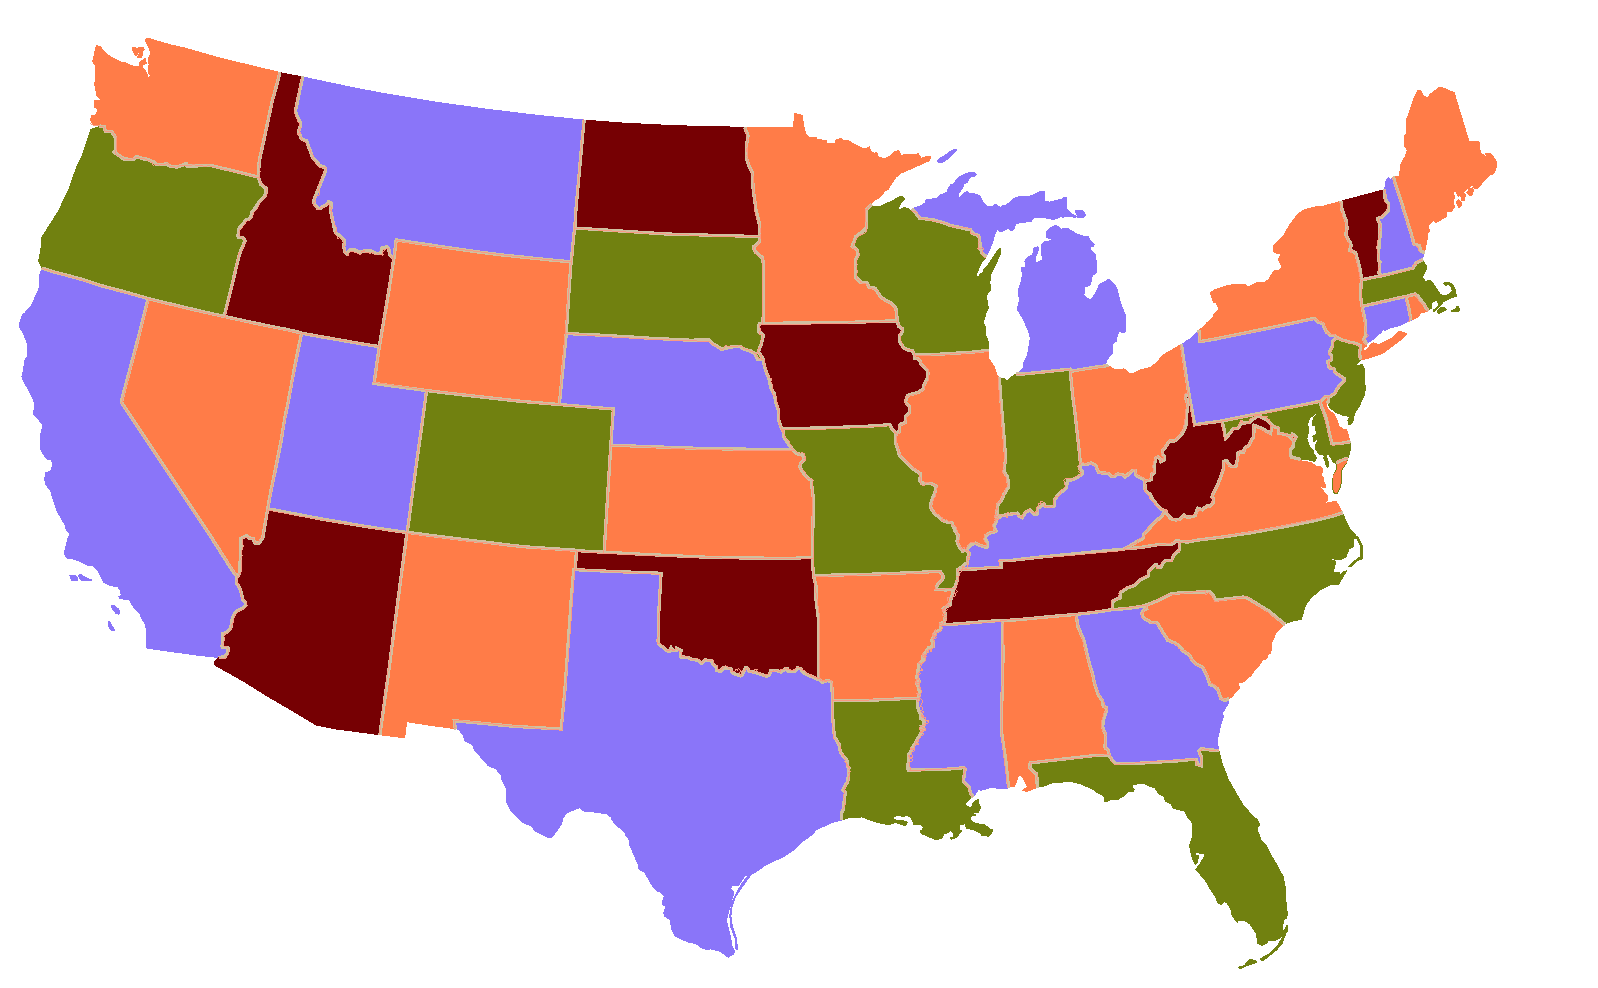
\includegraphics[width=14cm]{../figures/map-colors.pdf}
    \end{figure}
  \end{frame}

  \begin{frame}
    \frametitle{Overview}
    \begin{multicols}{2}
      \tableofcontents
    \end{multicols}
  \end{frame}

  \section{Background}

  \subsection{Graph Theory}

  \begin{frame}
    \frametitle{Graph Theory}



    \only<1-2>{
      \begin{textblock*}{\examplewidth}(0cm,\exampleheight) % {block width} (coords)
        \centering
        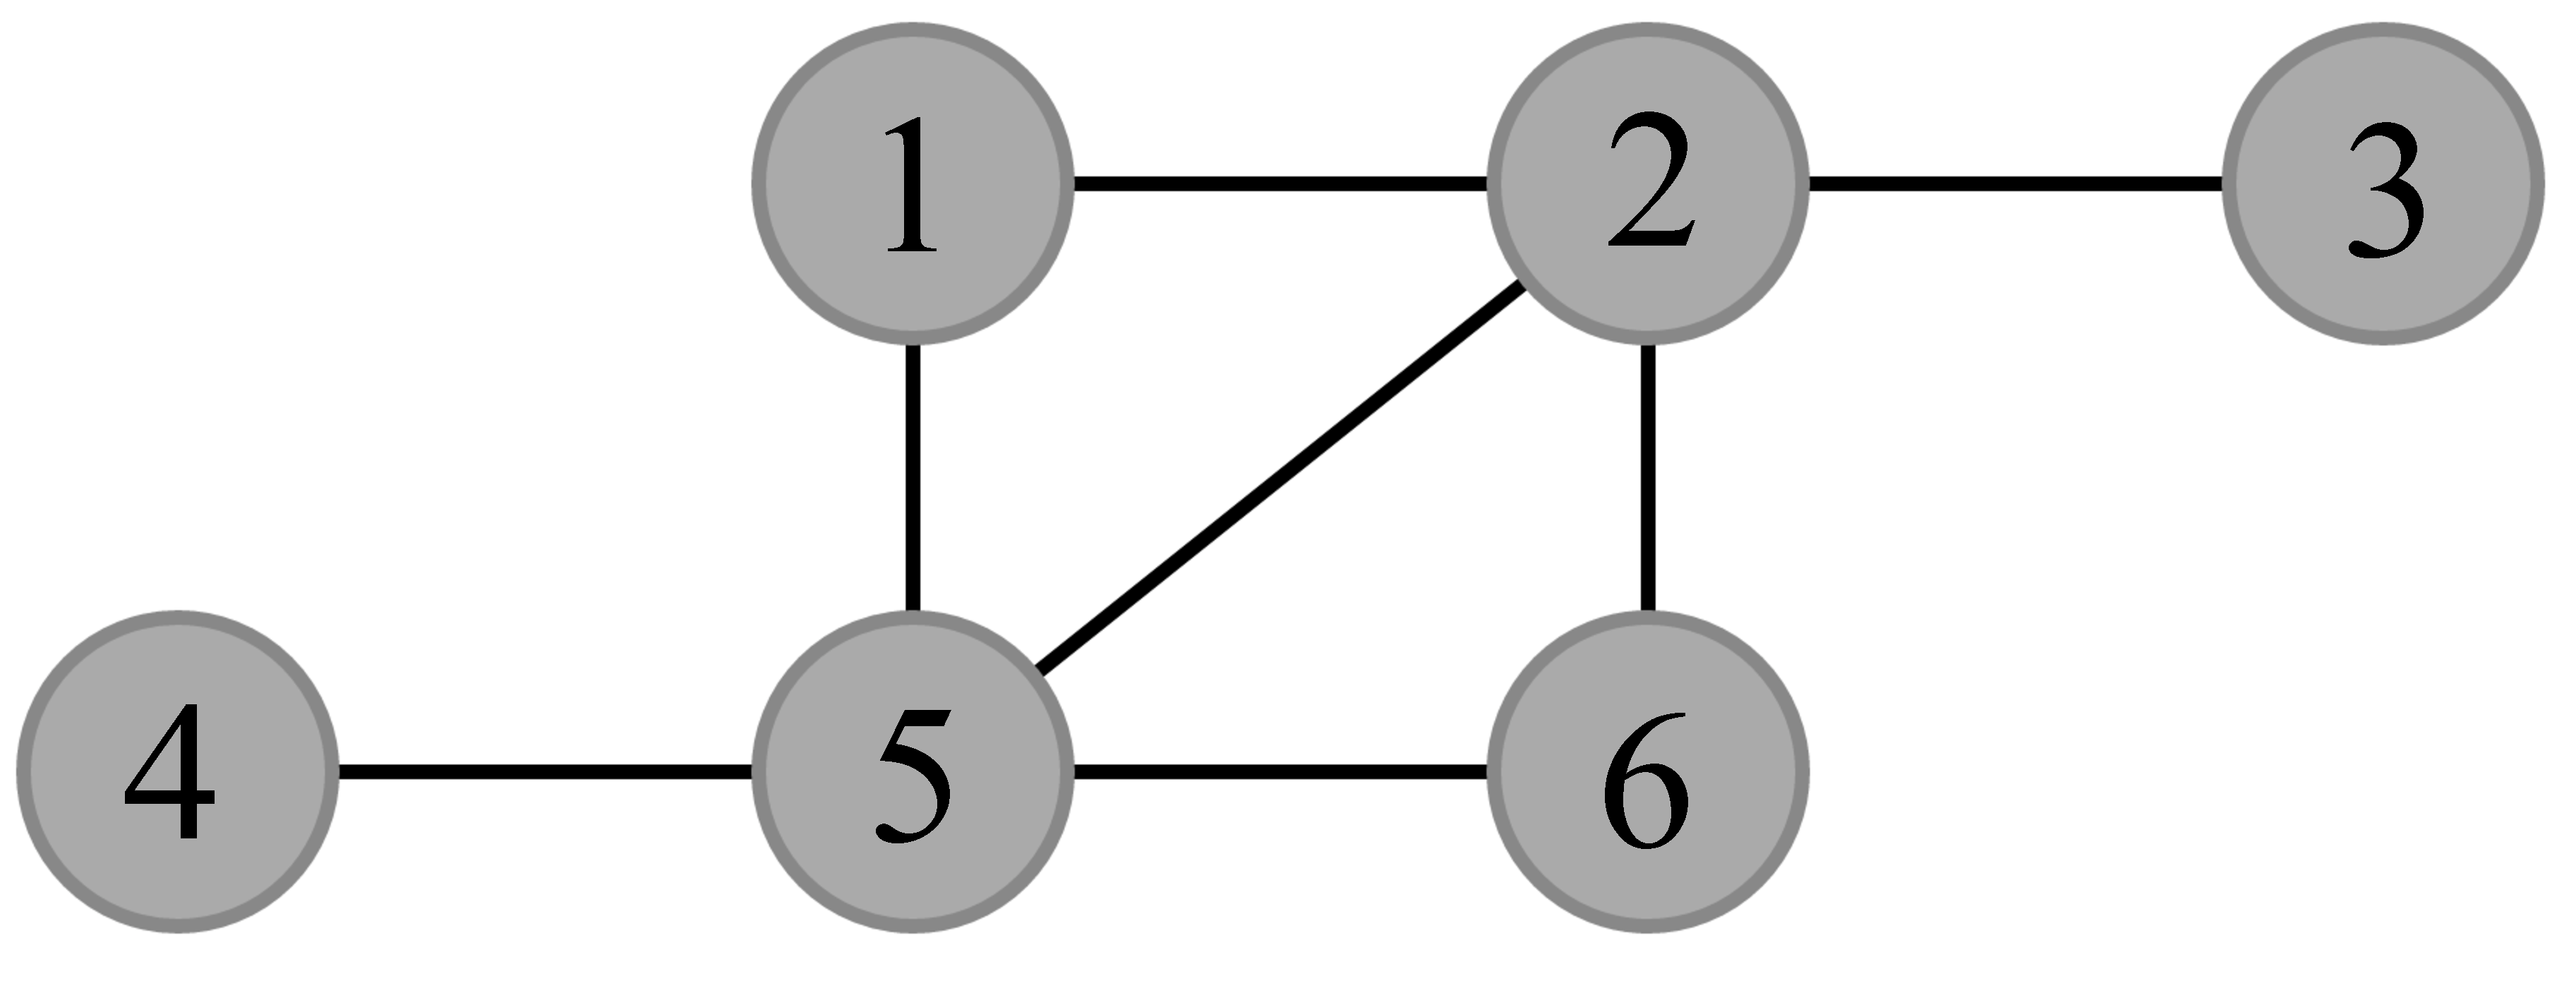
\includegraphics[width=8cm]{../figures/example.pdf}
      \end{textblock*}
    }

    \only<3> {
      \begin{textblock*}{\examplewidth}(0cm,\exampleheight) % {block width} (coords)
        \centering
        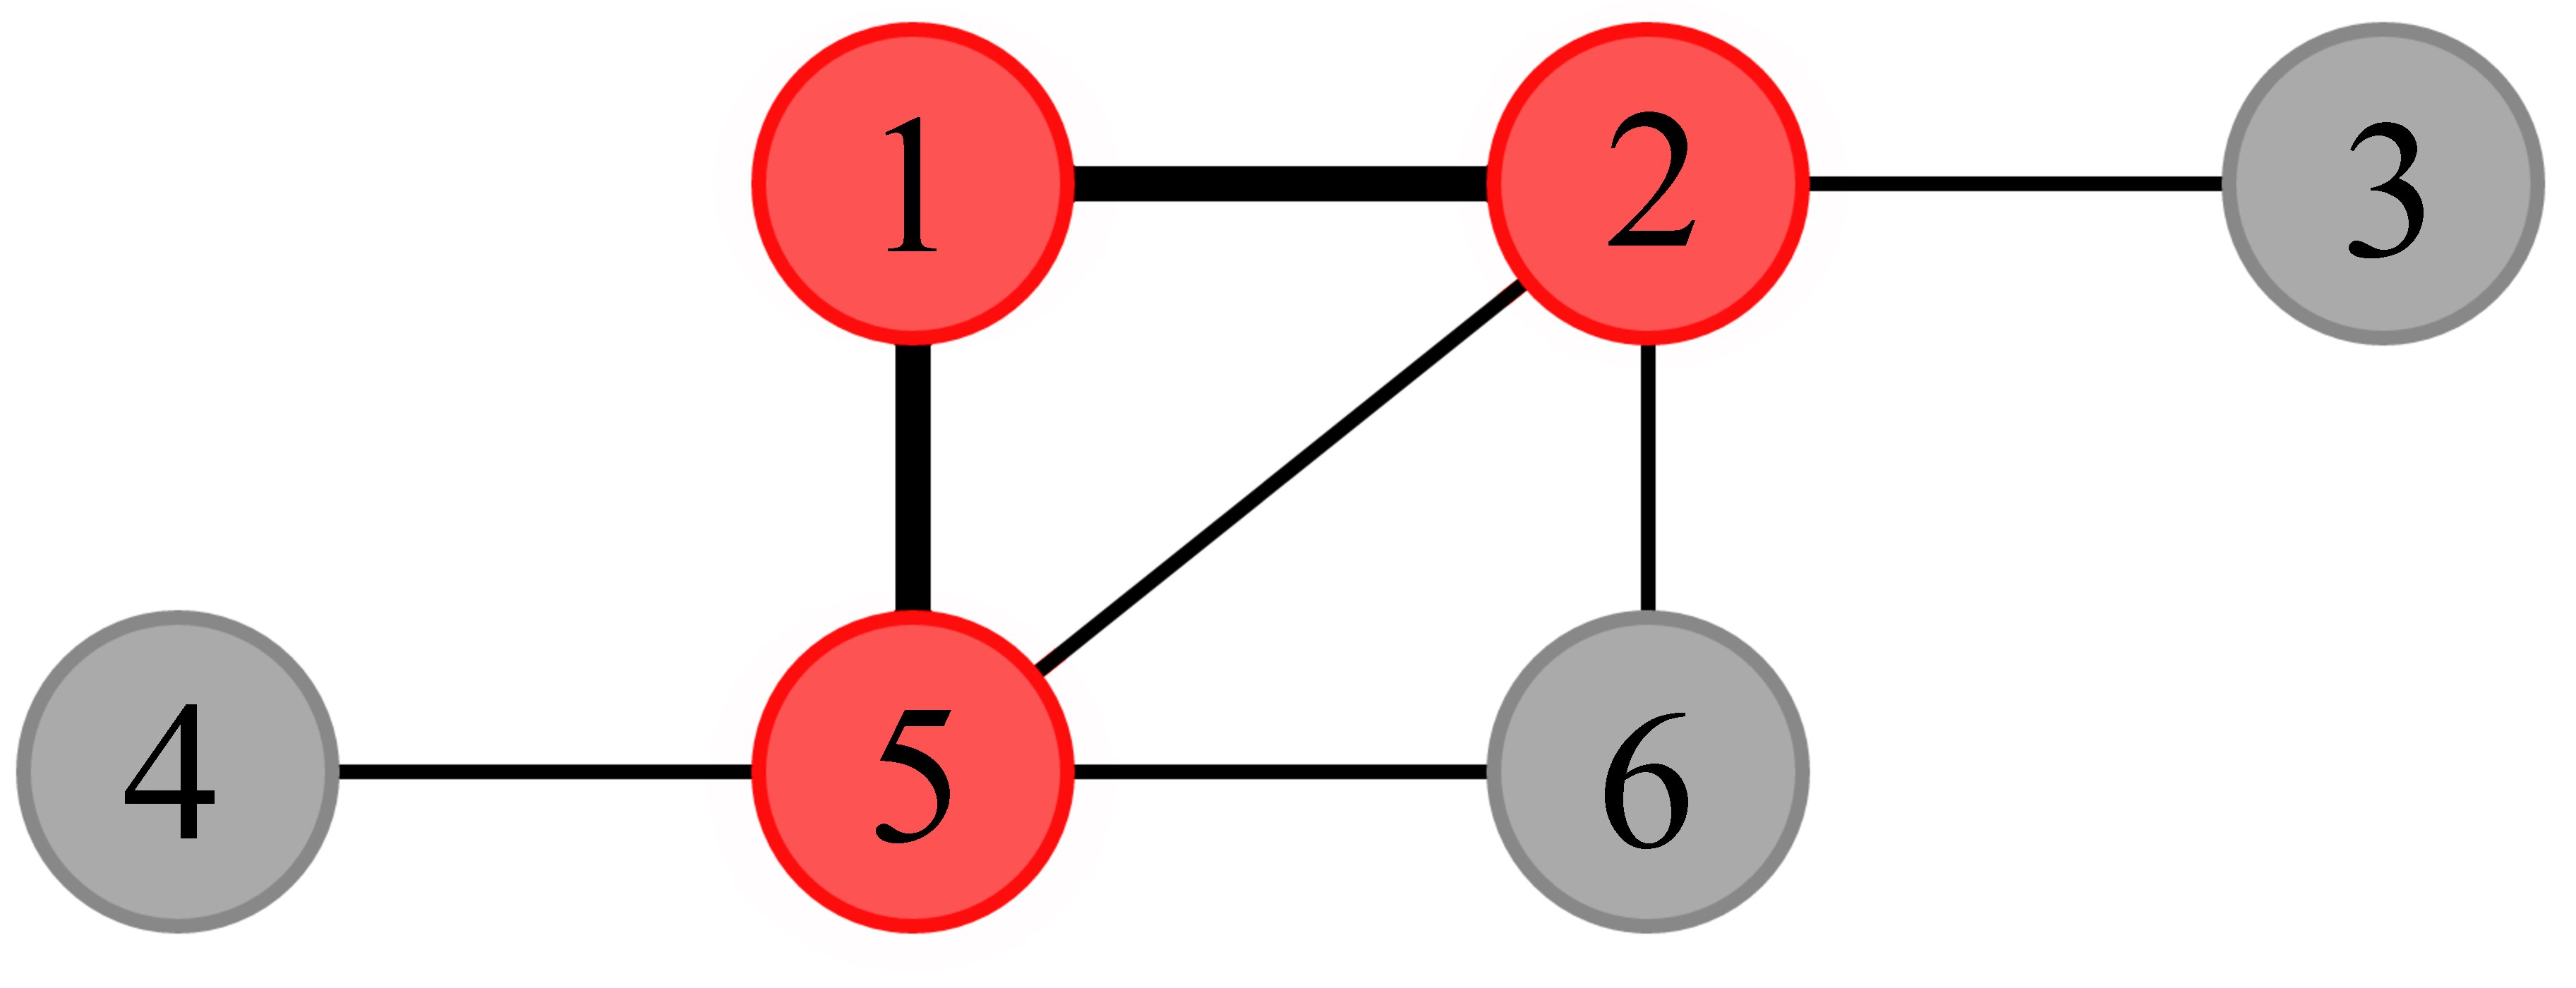
\includegraphics[width=8cm]{../figures/example-neighborhoods-1.pdf}
      \end{textblock*}
    }

    \only<4> {
      \begin{textblock*}{\examplewidth}(0cm,\exampleheight) % {block width} (coords)
        \centering
        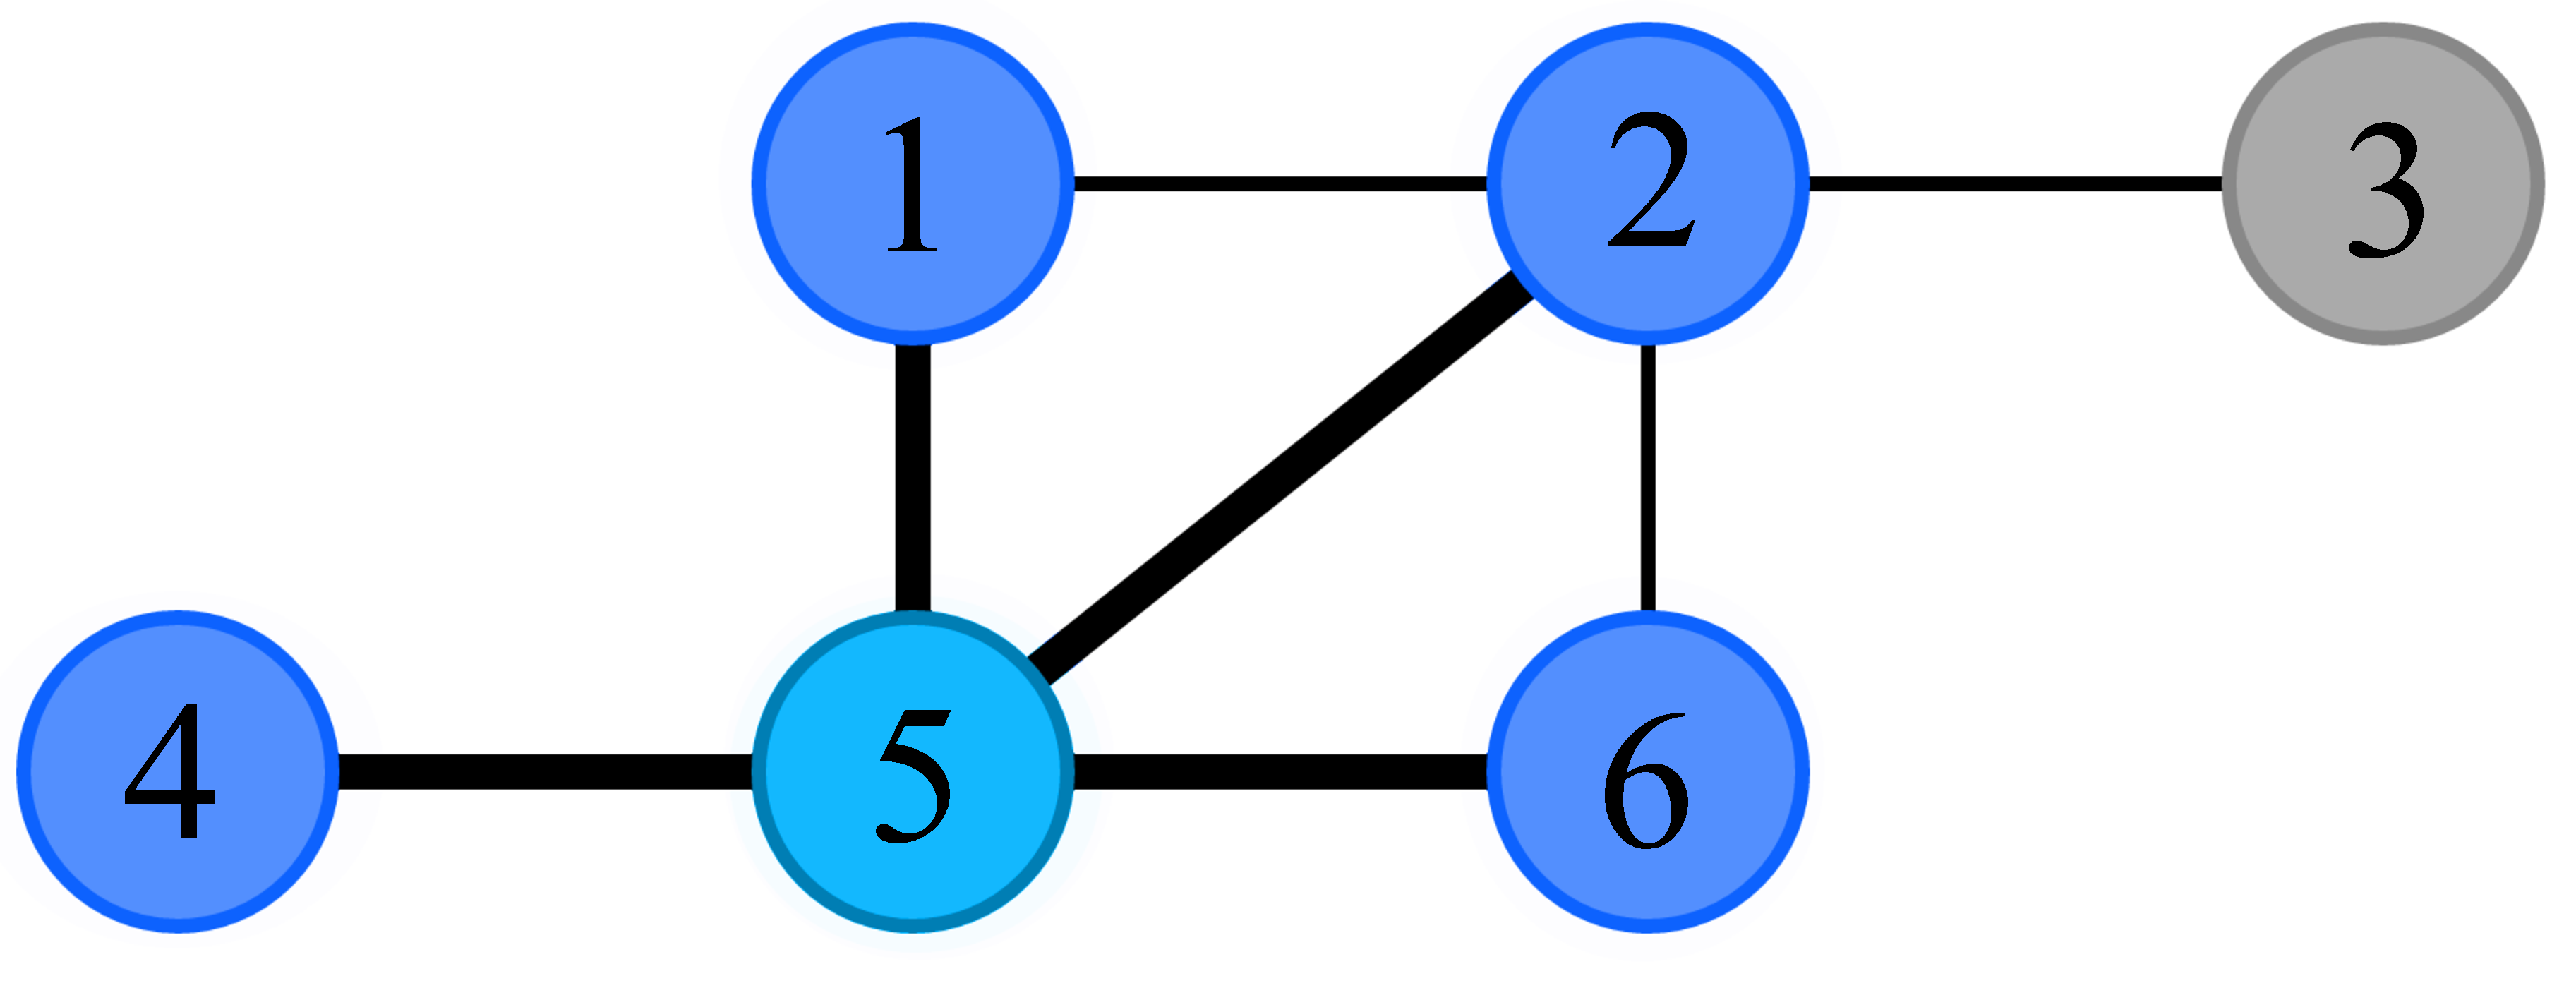
\includegraphics[width=8cm]{../figures/example-neighborhoods-2.pdf}
      \end{textblock*}
    }

    \vspace{4cm}

    \vfill

    \begin{itemize}
      \item<1-4> A \textbf{graph} is the set of vertices \emph{V} and a set of edges \emph{E}.
      \item<2-4> The \textbf{neighborhood} of a vertex $v$ is a set of all vertices adjacent to $v$ plus $v$ itself.
      \only<1-2>{\item<3> Example: The neighborhood of vertex 1: $\{1, 2, 5\}$.}
      \only<3>{\item<3> Example: The neighborhood of vertex 1: $\{1, 2, 5\}$.}
      \only<4>{\item<4> Example: The neighborhood of vertex 5: $\{1, 2, 4, 5, 6\}$.}
    \end{itemize}

  \end{frame}

  \subsection{Graph Coloring}

  \begin{frame}
    \frametitle{Vertex Coloring}

    \begin{textblock*}{\examplewidth}(0cm,\exampleheight) % {block width} (coords)
      \centering
      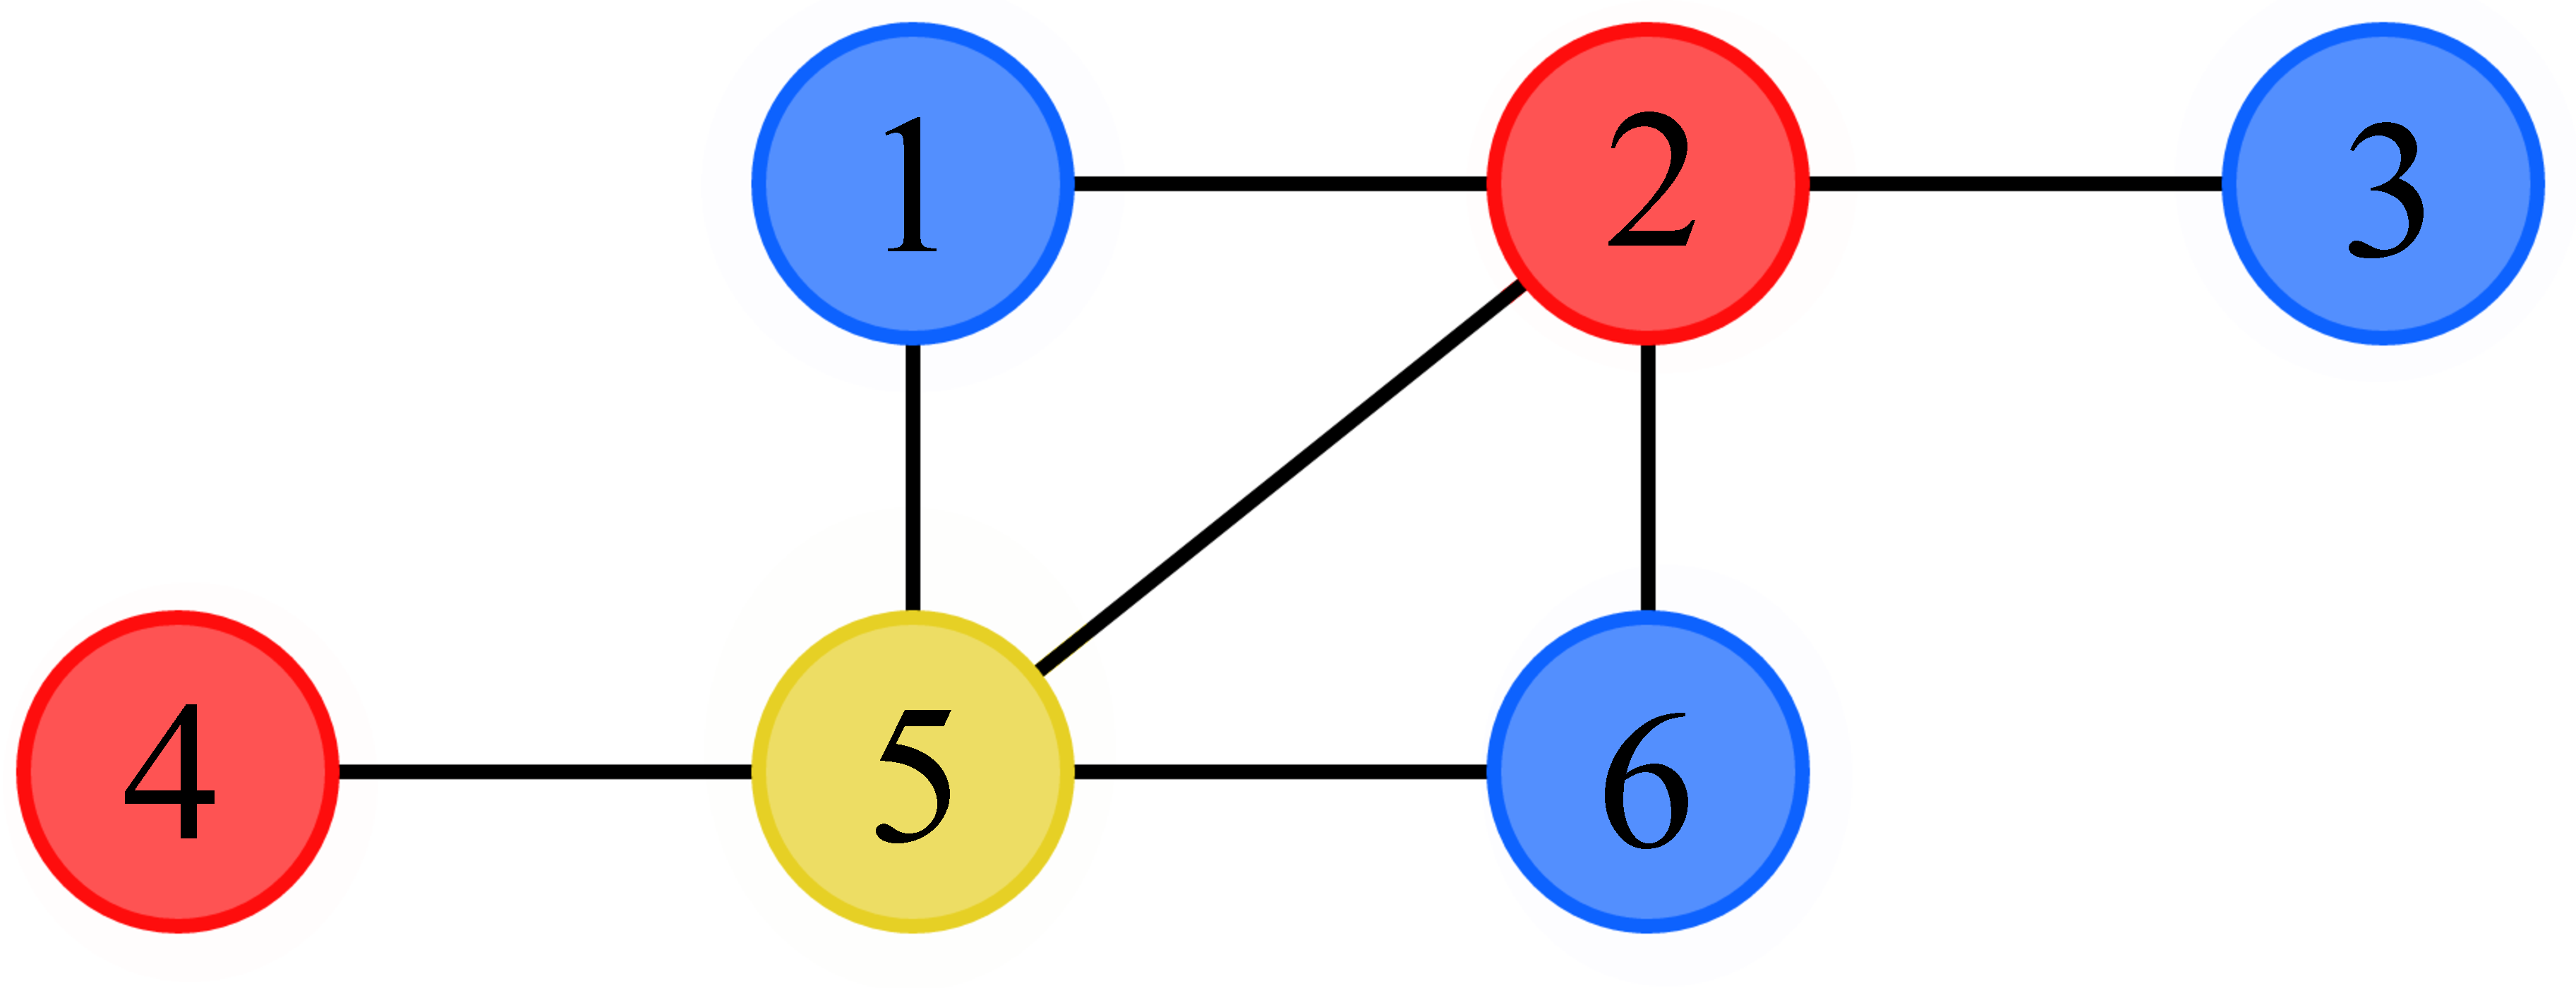
\includegraphics[width=8cm]{../figures/example-vcp.pdf}
    \end{textblock*}

    \vspace{4cm}
    \vfill

    \begin{itemize}
      \item A proper \textbf{vertex coloring} of a graph $G$ assigns colors to \emph{every} vertex such that no two adjacent vertices share the same color.
      \item The \textbf{chromatic number} of $G$ is the minimum number of colors needed to properly color $G$.
    \end{itemize}
  \end{frame}

  \begin{frame}
    \frametitle{Conflict-Free Coloring}

    \begin{textblock*}{\examplewidth}(0cm,\exampleheight) % {block width} (coords)
      \centering
      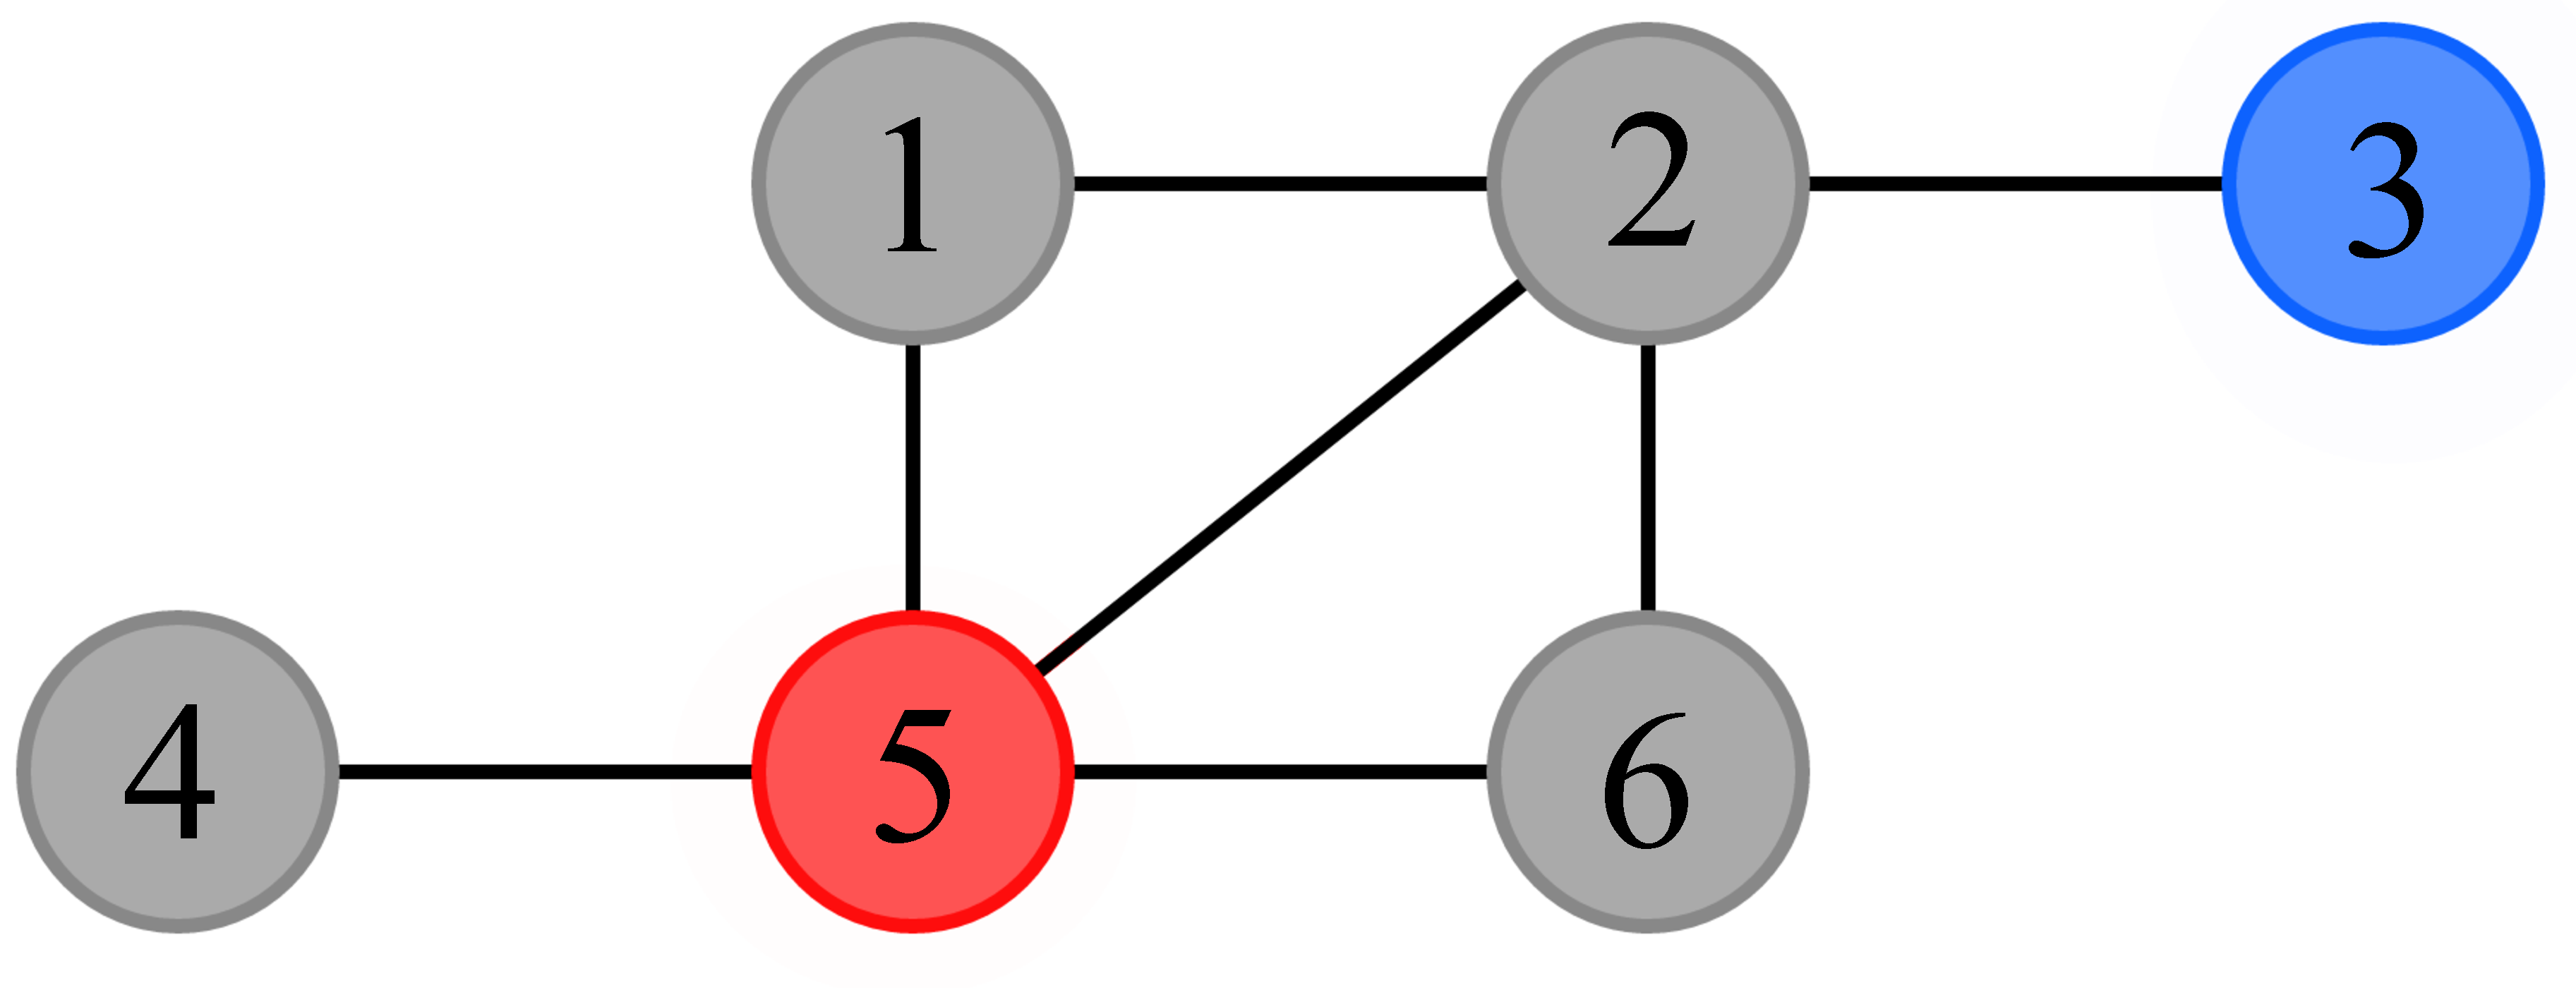
\includegraphics[width=8cm]{../figures/example-cfcp.pdf}
    \end{textblock*}

    \vspace{4cm}
    \vfill

    \begin{itemize}
      \item<1-2> A \textbf{conflict-free coloring} of a graph $G$ assigns colors to \emph{some} vertices such that there is a uniquely colored vertex within the neighborhood of every vertex.
      \item<2> Every proper vertex coloring of $G$ is also a conflict-free coloring of $G$ as every vertex $v$ would be a unique color itself in its neighborhood.
    \end{itemize}
  \end{frame}

  \begin{frame}
    \frametitle{Conflict-Free Coloring}

    \begin{textblock*}{\examplewidth/2}(0cm,\exampleheight) % {block width} (coords)
      \centering
      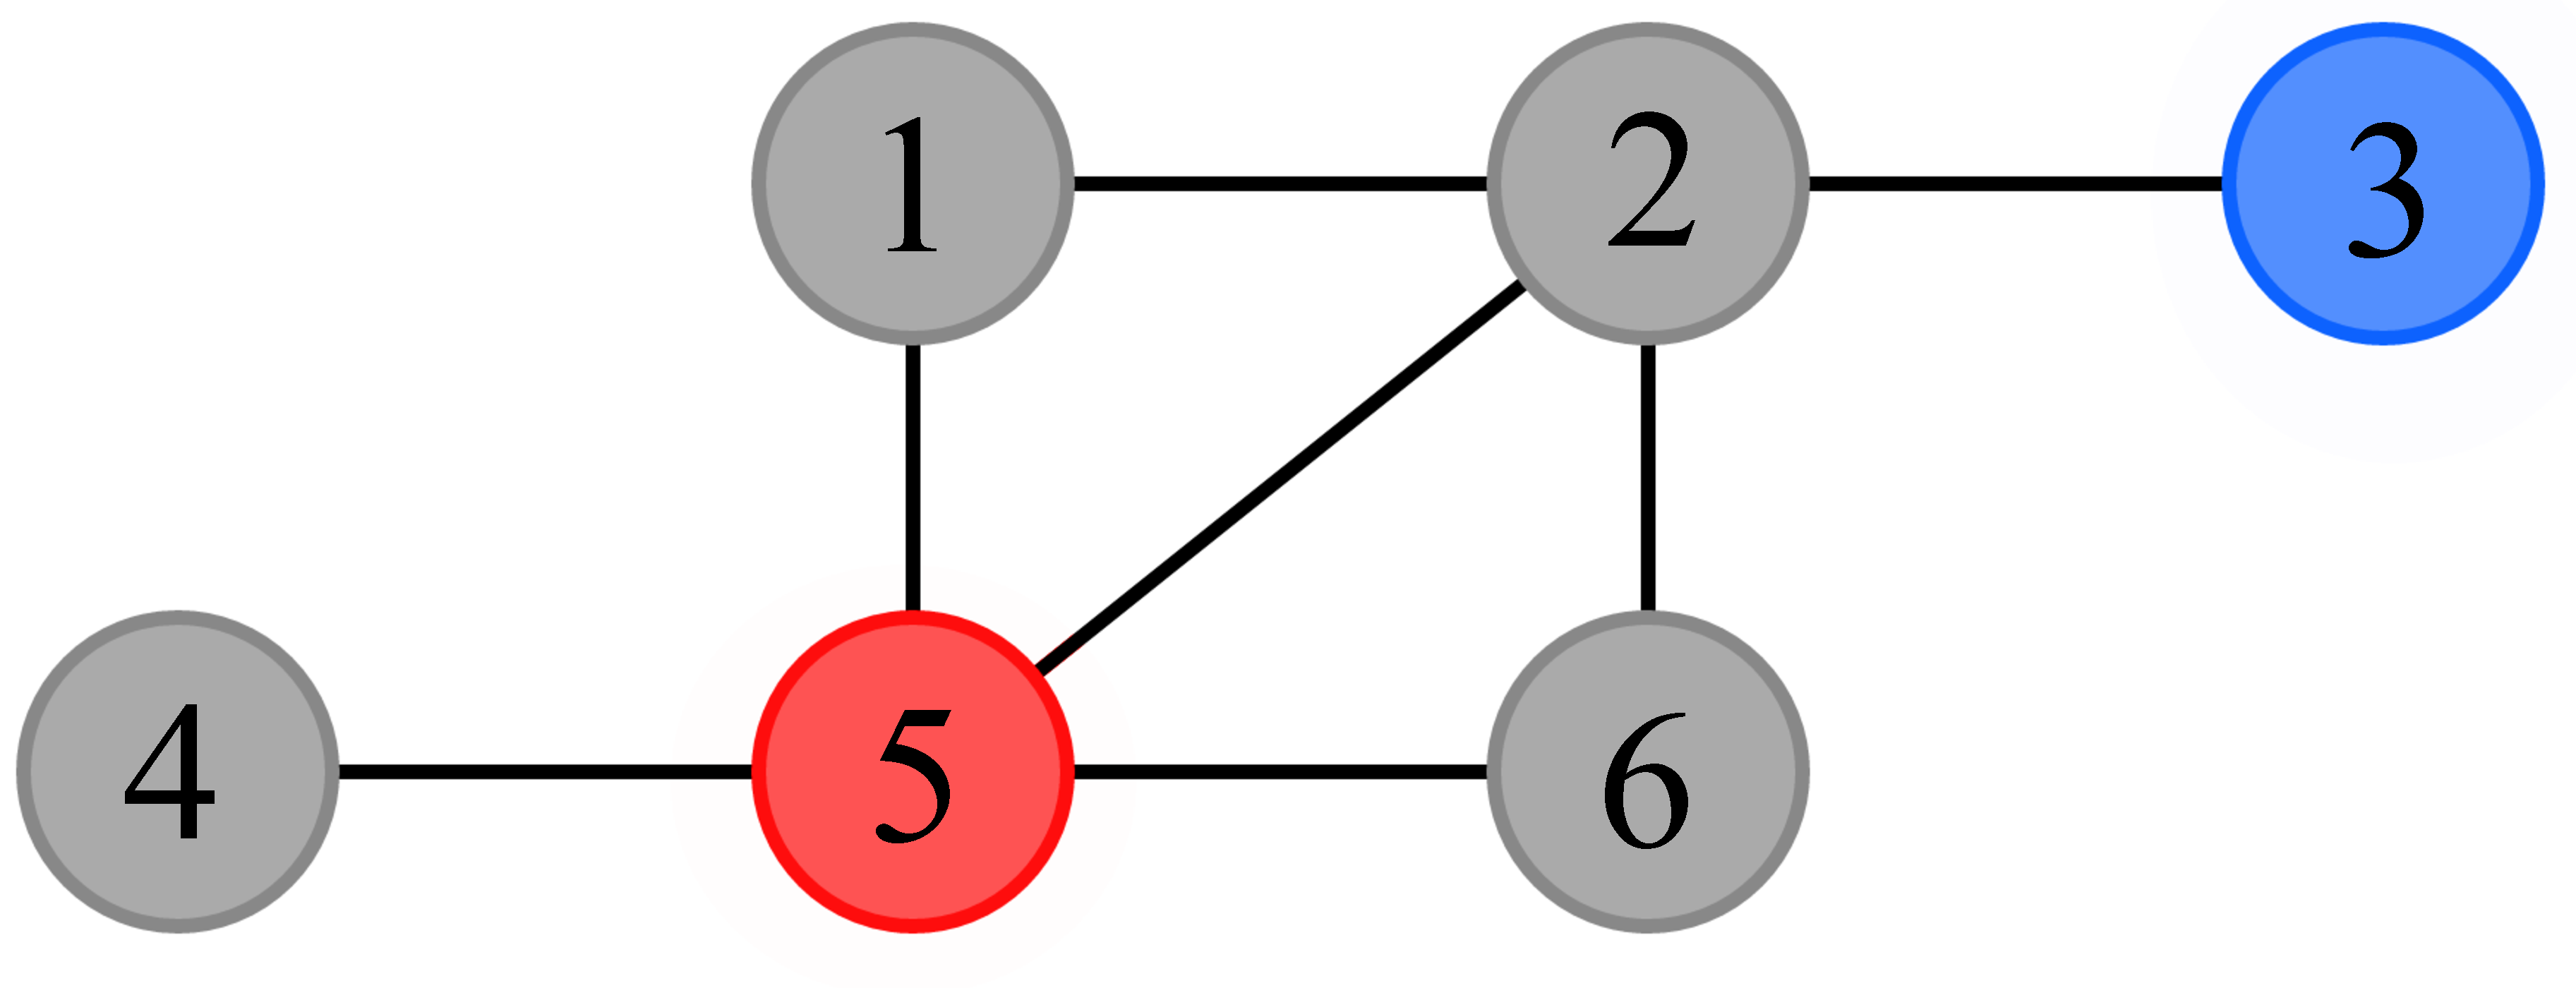
\includegraphics[width=6.5cm]{../figures/example-cfcp.pdf}
    \end{textblock*}

    \begin{textblock*}{\examplewidth/2}(8cm,\exampleheight) % {block width} (coords)
      \centering
      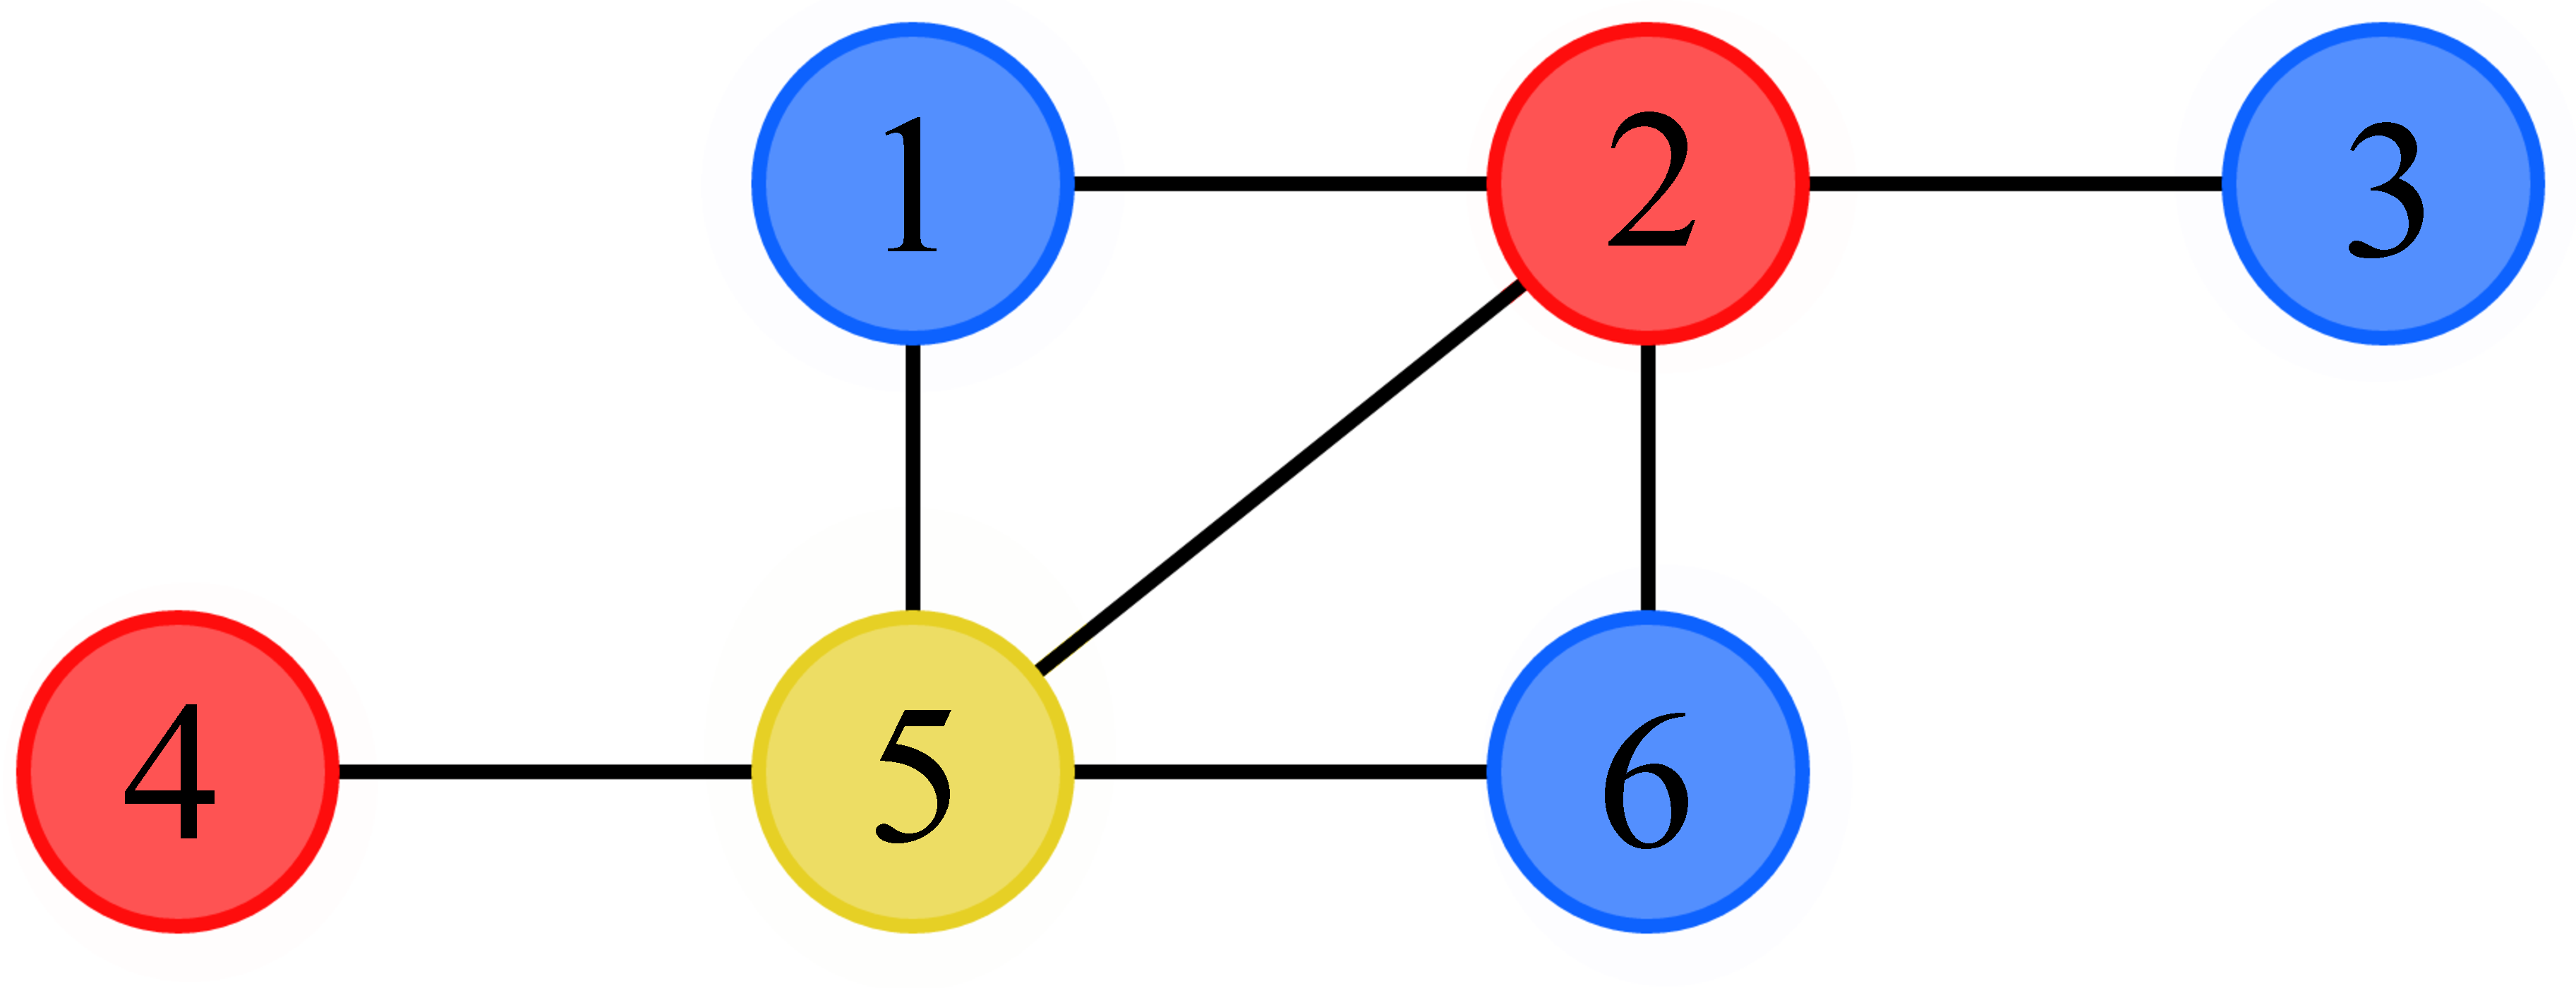
\includegraphics[width=6.5cm]{../figures/example-vcp.pdf}
    \end{textblock*}

    \vspace{3cm}

    \begin{center}
      Every vertex $v$ has at least one unique color within its neighborhood.
    \end{center}

    \pause

    \begin{columns}
      \begin{column}{0.5\textwidth}
        \begin{itemize}[leftmargin=1.4cm]
          \item[$v$ = 1:] $\{1: none,\ 2: none,\ 5: \textbf{red}\}$
          \item[$v$ = 2:] $\{1: none,\ 2: none,\ 3: \textbf{blue},$ \newline $\quad 5: red,\ 6: none\}$
          \item[$v$ = 3:] $\{2: none,\ 3: \textbf{blue}\}$
        \end{itemize}
      \end{column}

      \pause

      \begin{column}{0.5\textwidth}
        \begin{itemize}[leftmargin=1.4cm]
          \item[$v$ = 1:] $\{1: \textbf{blue},\ 2: red,\ 5: yellow\}$
          \item[$v$ = 2:] $\{1: blue,\ 2: \textbf{red},\ 3: blue,$ \newline $\quad 5: yellow,\ 6: blue\}$
          \item[$v$ = 3:] $\{2: red,\ 3: \textbf{blue}\}$
        \end{itemize}
      \end{column}
    \end{columns}

  \end{frame}

  \begin{frame}
    \frametitle{Conflict-Free Coloring Examples}

    \begin{textblock*}{\examplewidth}(1cm,\exampleheight) % {block width} (coords)
      Incorrect conflict-free colorings and their fixes:
    \end{textblock*}

    \vspace{0.5cm}

    \pause

    \begin{columns}
      \begin{column}{0.33333\textwidth}
        \only<2>{
          \begin{figure}[h]
            \centering
            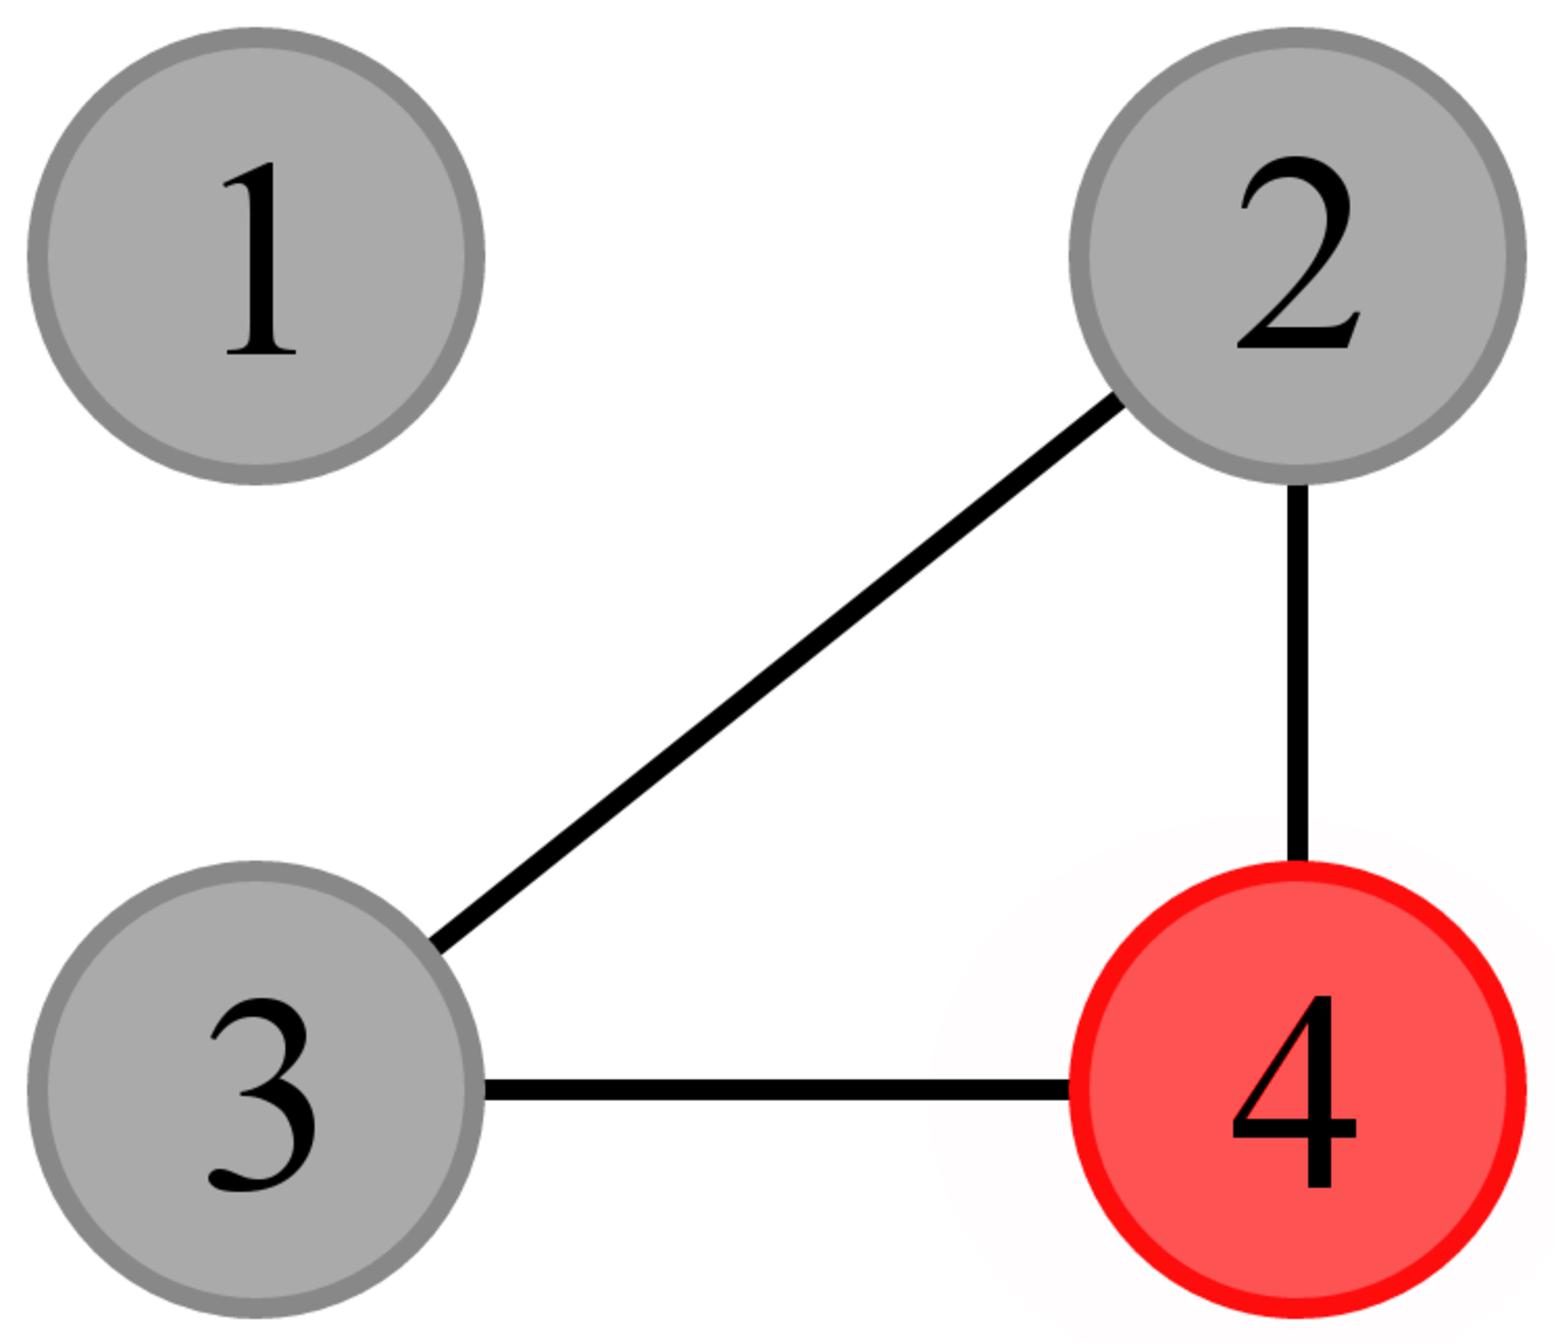
\includegraphics[width=3cm]{../figures/examples-1-incorrect-1.pdf}
          \end{figure}
        }

        \only<3-7>{
          \begin{figure}[h]
            \centering
            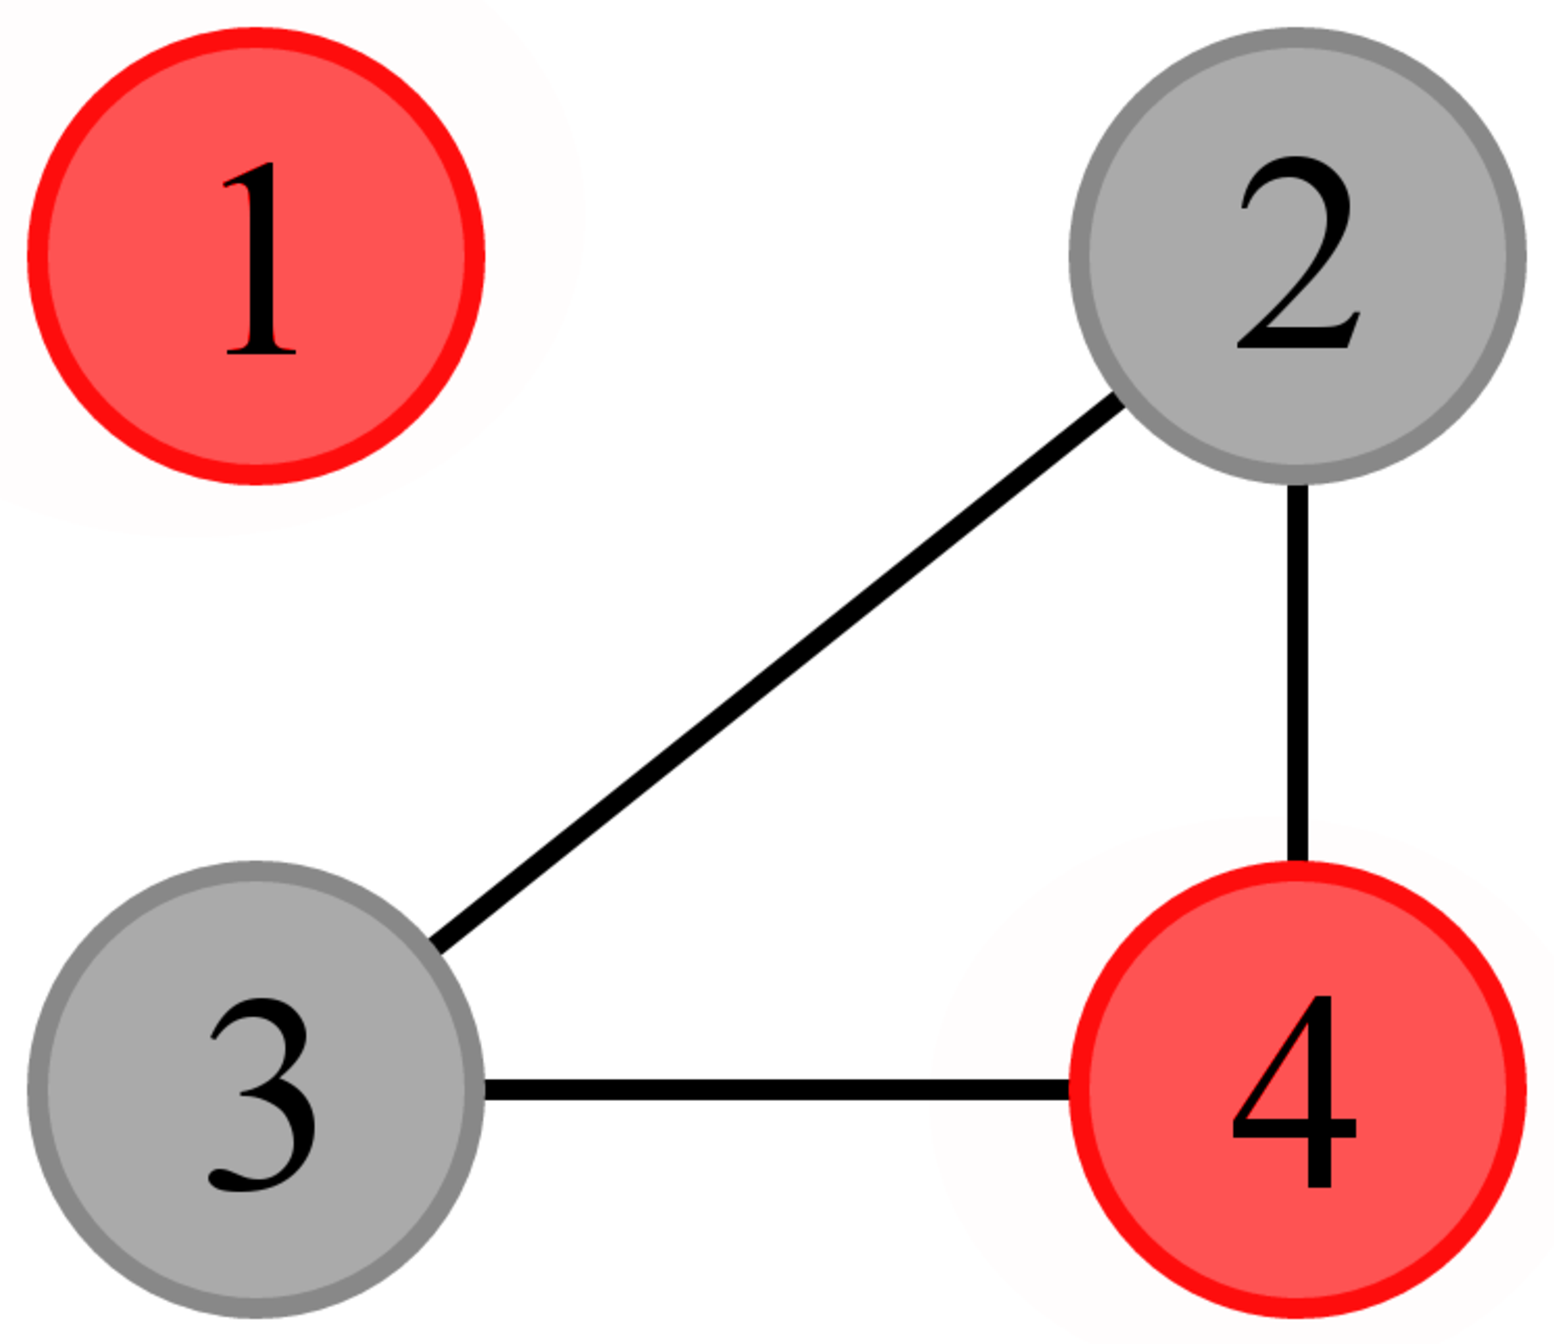
\includegraphics[width=3cm]{../figures/examples-1-incorrect-1-corrected.pdf}
          \end{figure}
        }

        \centering
        Vertex 1 does not have a unique color in its neighborhood.
      \end{column}

      \pause
      \pause

      \begin{column}{0.33333\textwidth}

        \only<4>{
        \begin{figure}[h]
          \centering
          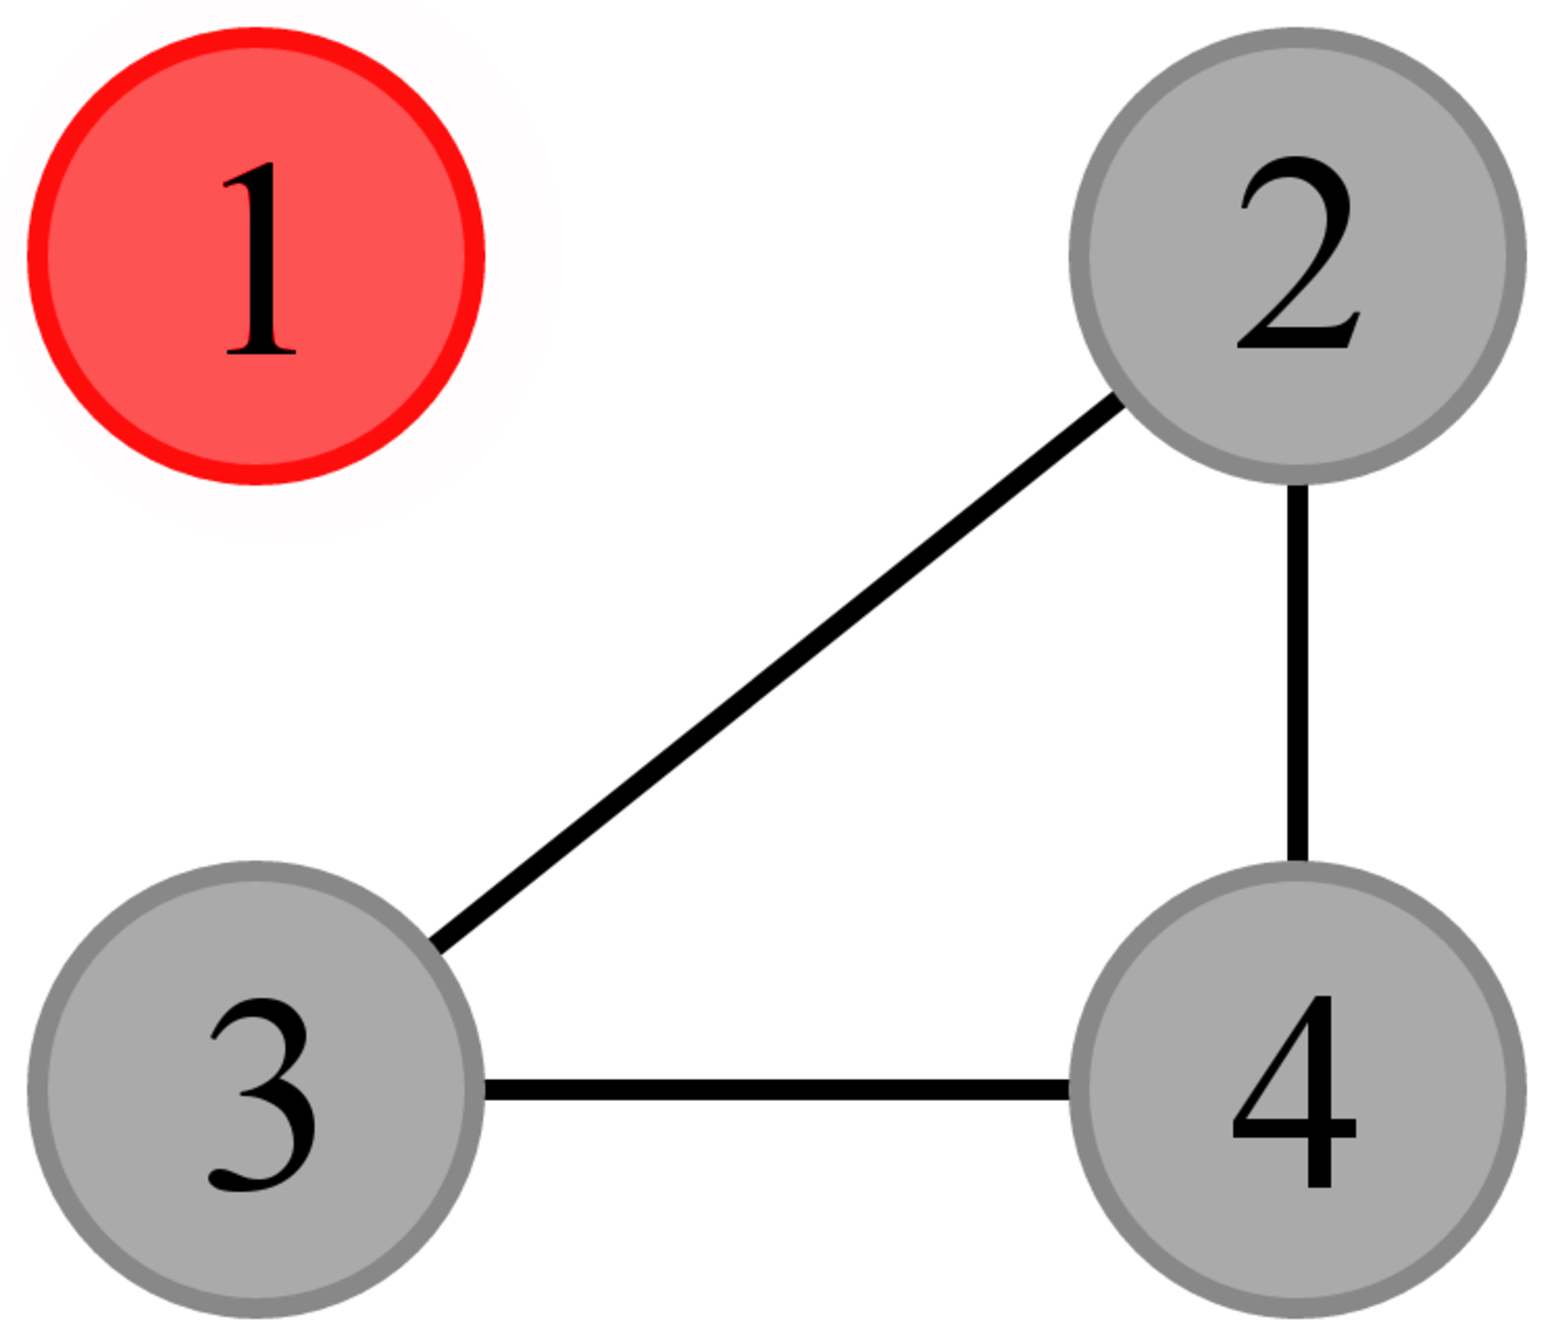
\includegraphics[width=3cm]{../figures/examples-1-incorrect-2.pdf}
        \end{figure}
        }

        \only<5-7>{
        \begin{figure}[h]
          \centering
          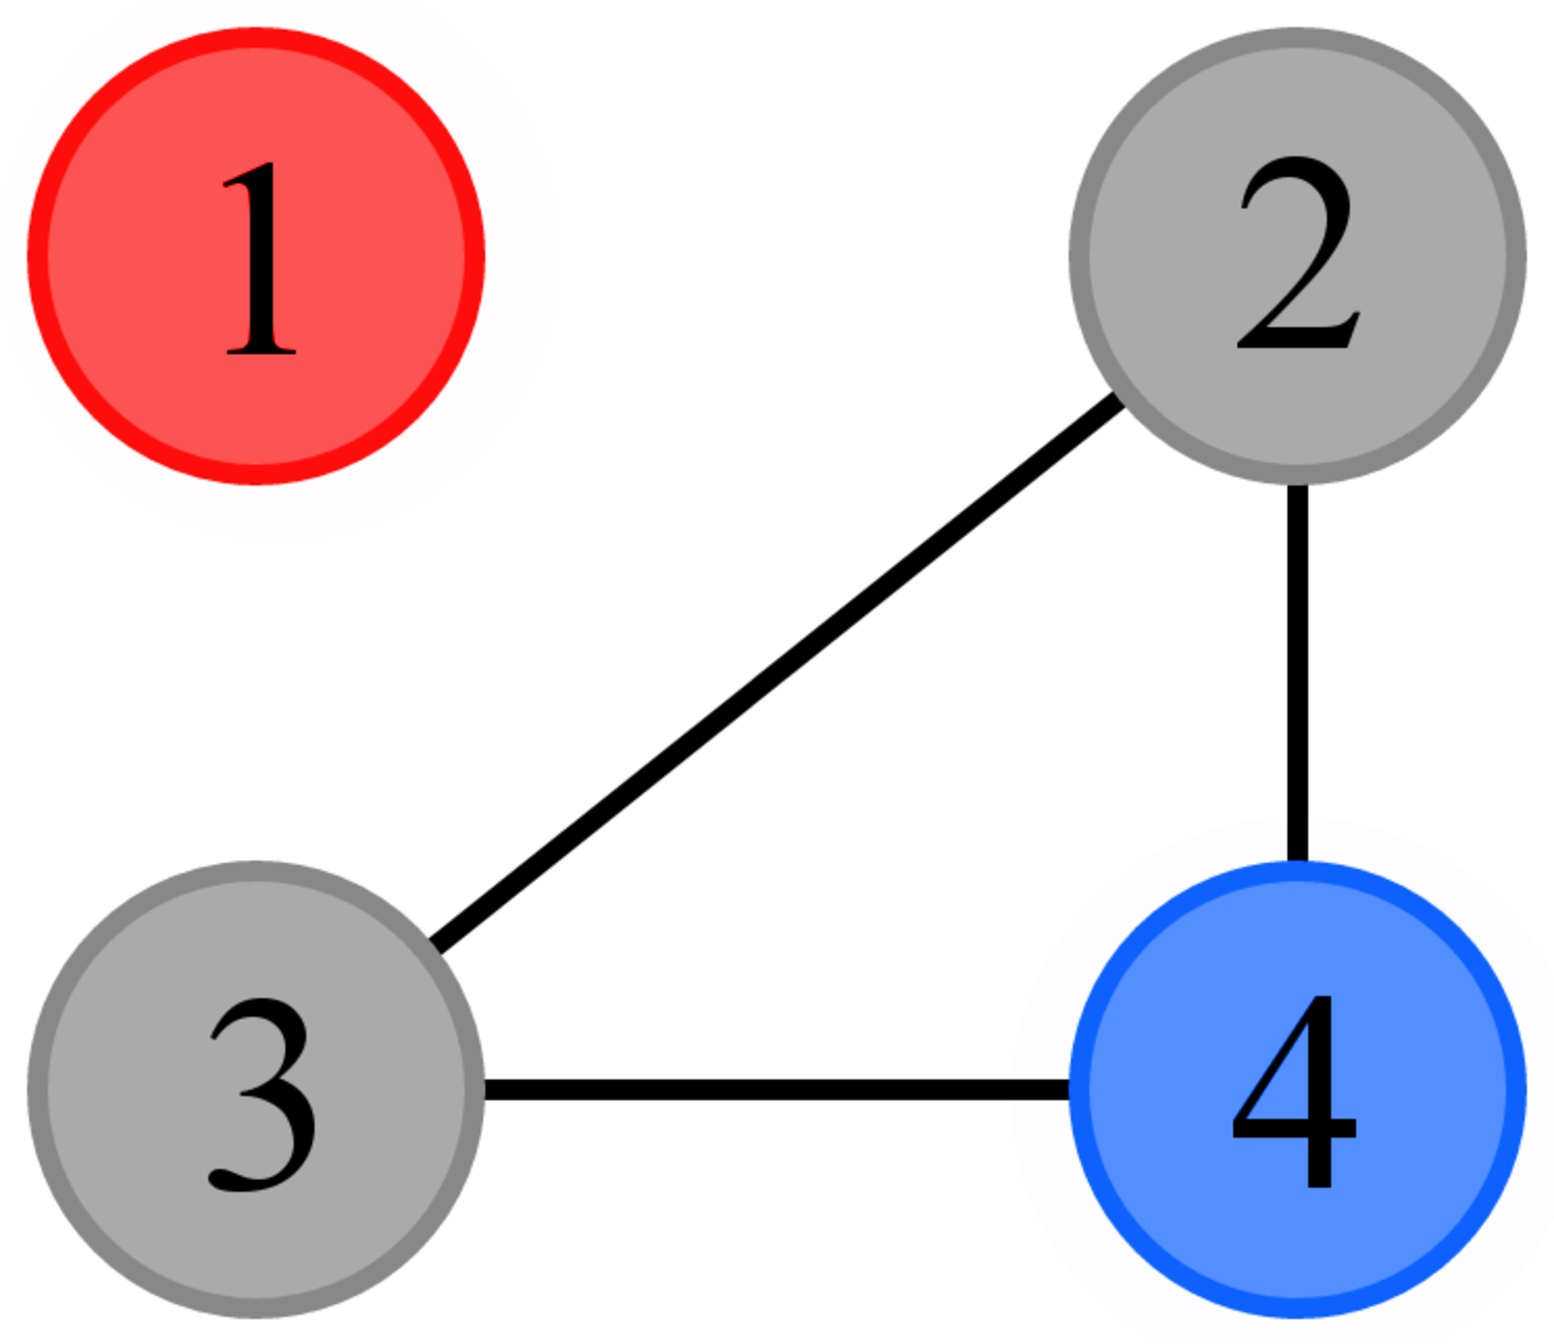
\includegraphics[width=3cm]{../figures/examples-1-incorrect-2-corrected.pdf}
        \end{figure}
        }

        \centering
        Vertices $\{2, 3, 4\}$ do not have a unique color in their neighborhoods.
      \end{column}

      \pause
      \pause

      \begin{column}{0.33333\textwidth}

        \only<6>{
        \begin{figure}[h]
          \centering
          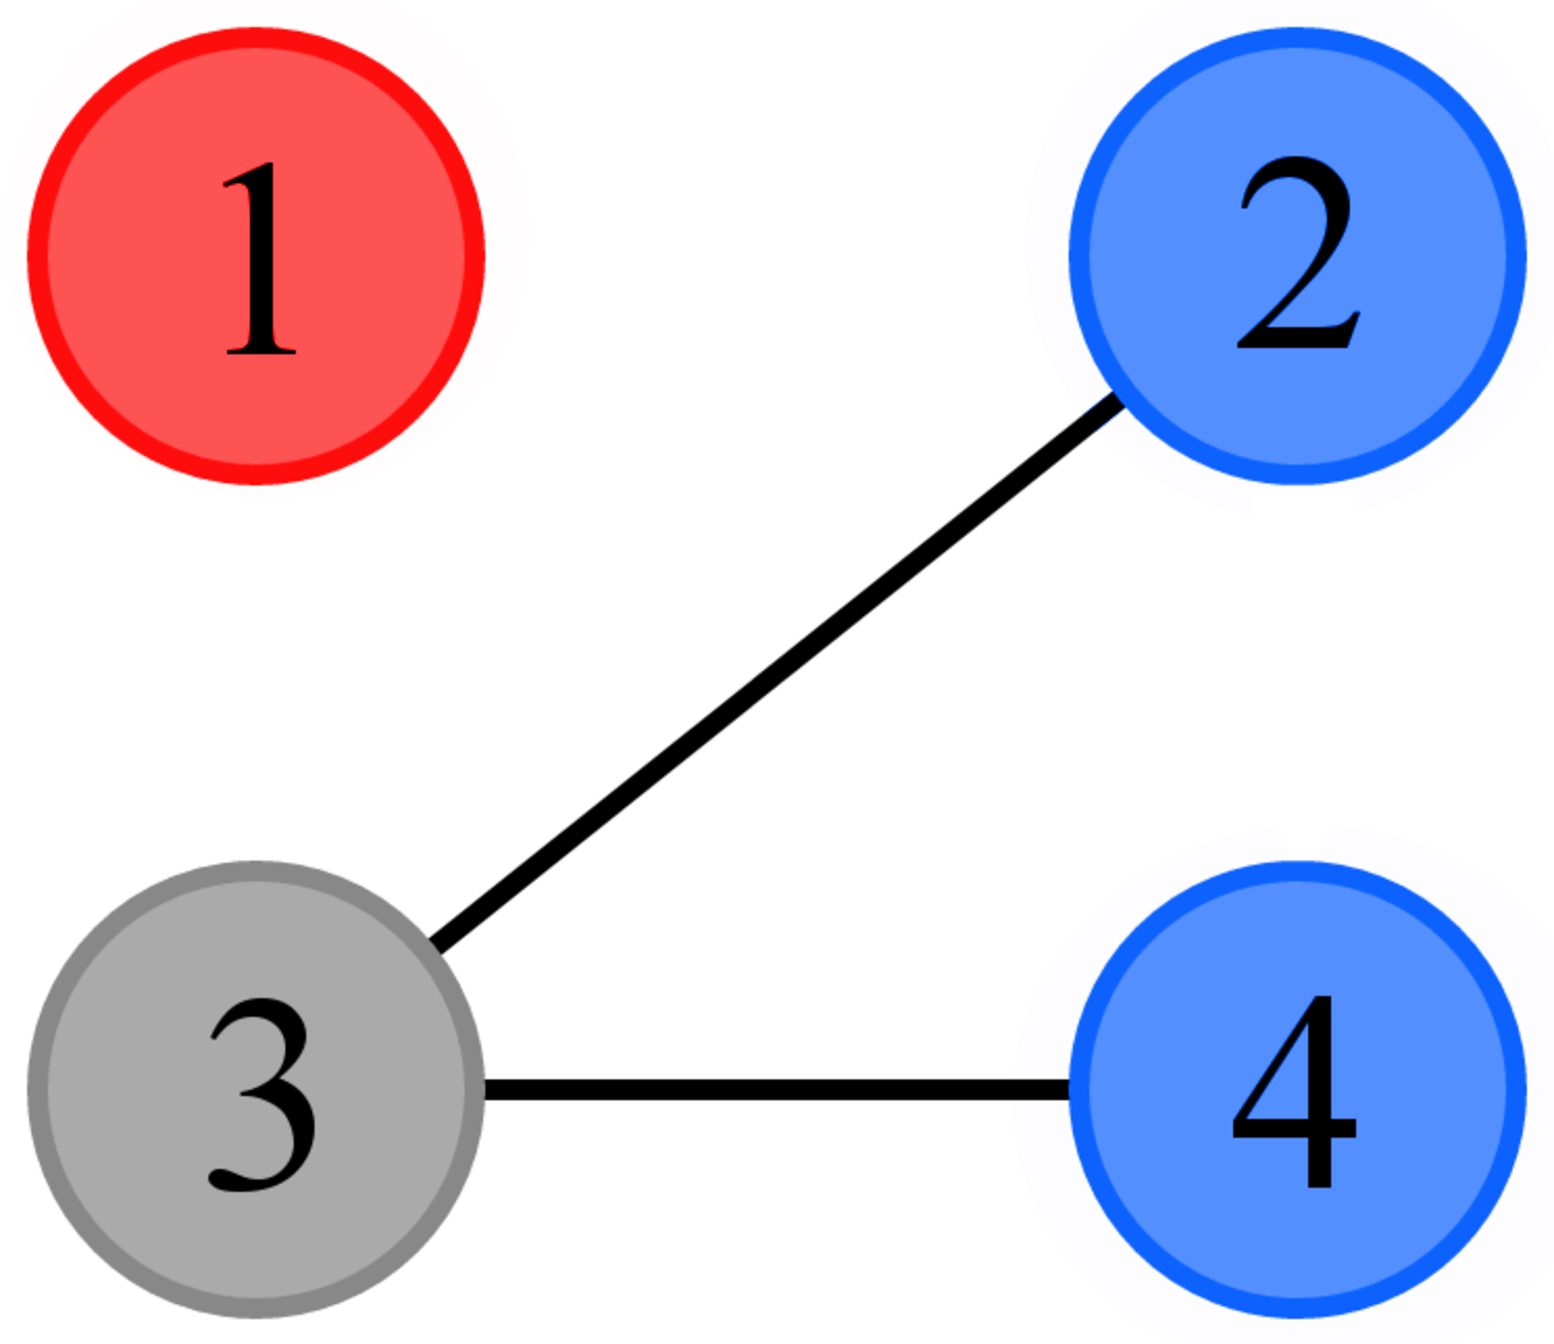
\includegraphics[width=3cm]{../figures/examples-1-incorrect-3.pdf}
        \end{figure}
        }

        \only<7>{
        \begin{figure}[h]
          \centering
          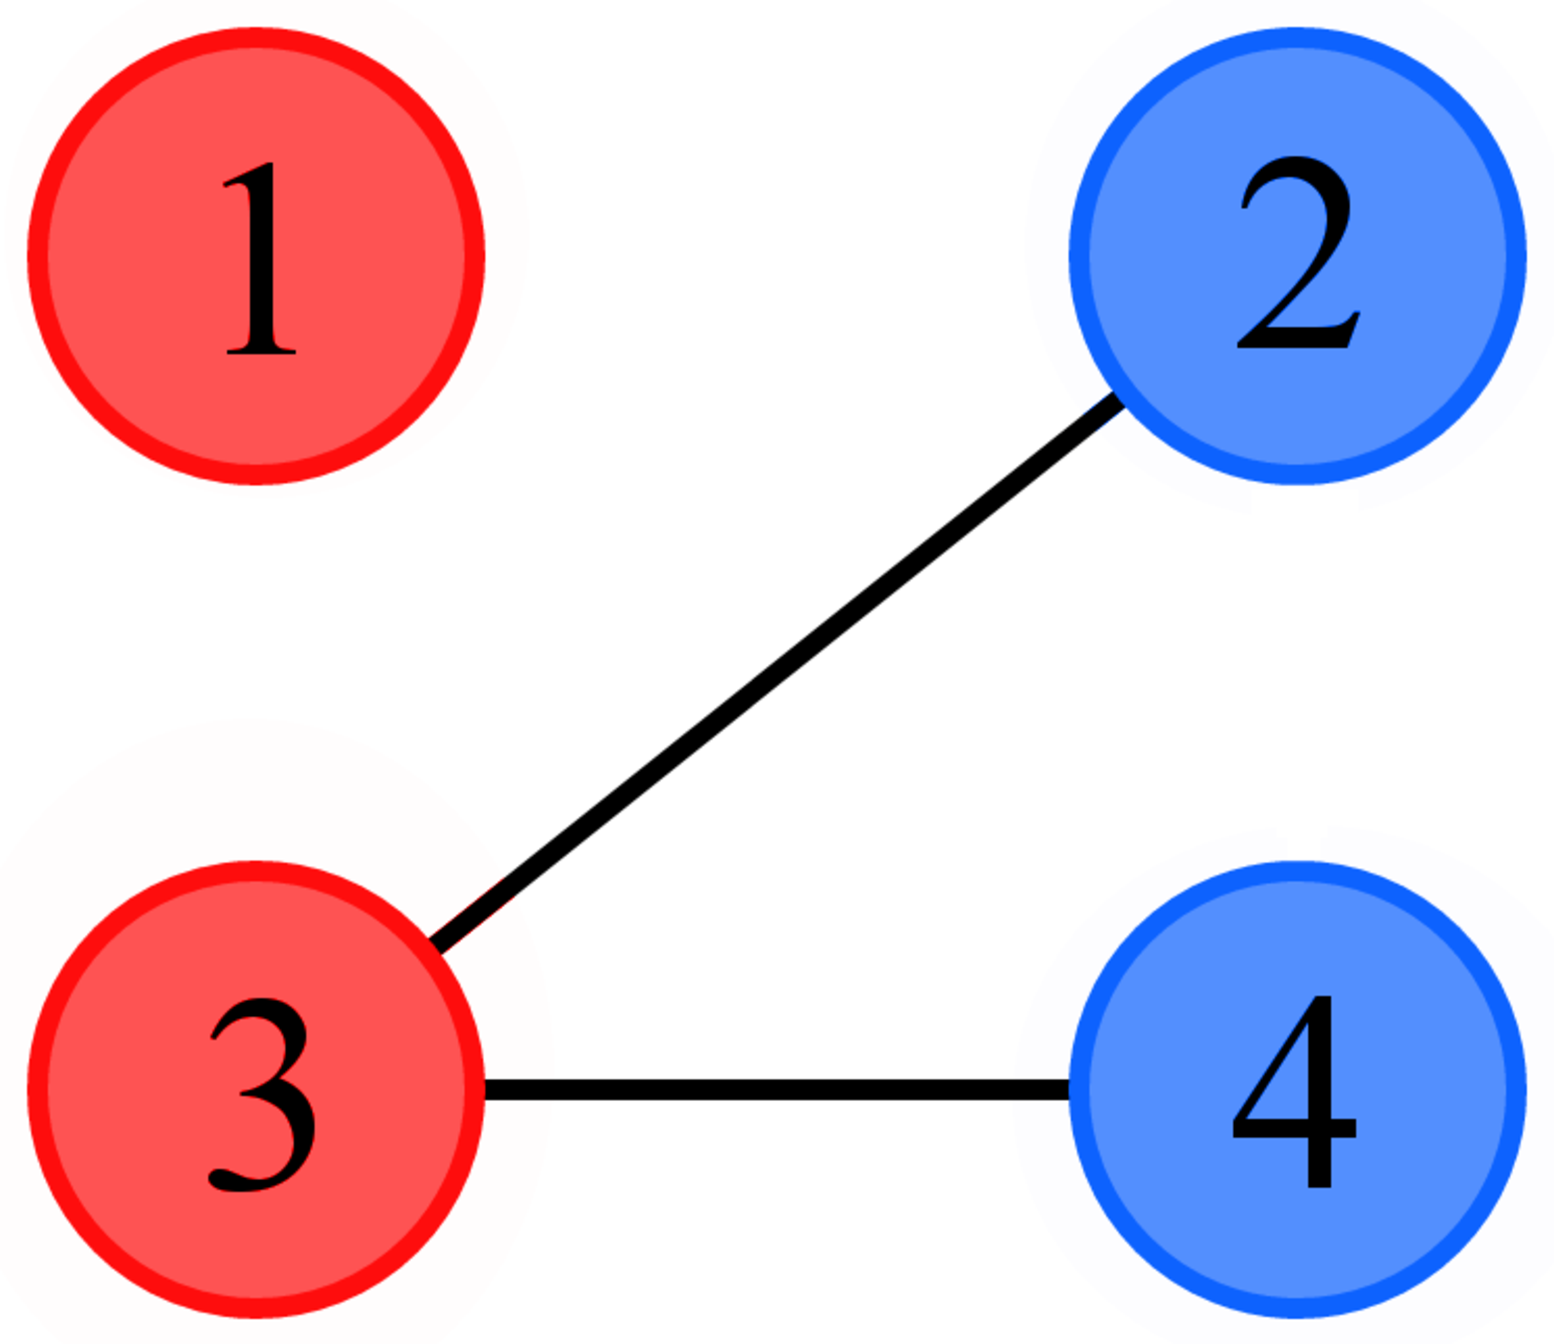
\includegraphics[width=3cm]{../figures/examples-1-incorrect-3-corrected.pdf}
        \end{figure}
        }

        \centering
        Vertex 3 does not have a unique color in its neighborhood.
      \end{column}
    \end{columns}

    % \begin{textblock*}{\examplewidth}(0cm,1.3cm) % {block width} (coords)
    %   \centering
    %   \textbf{Incorrect} colorings
    % \end{textblock*}
    %
    % \begin{textblock*}{\examplewidth}(0cm,2cm) % {block width} (coords)
    %   \centering
    %   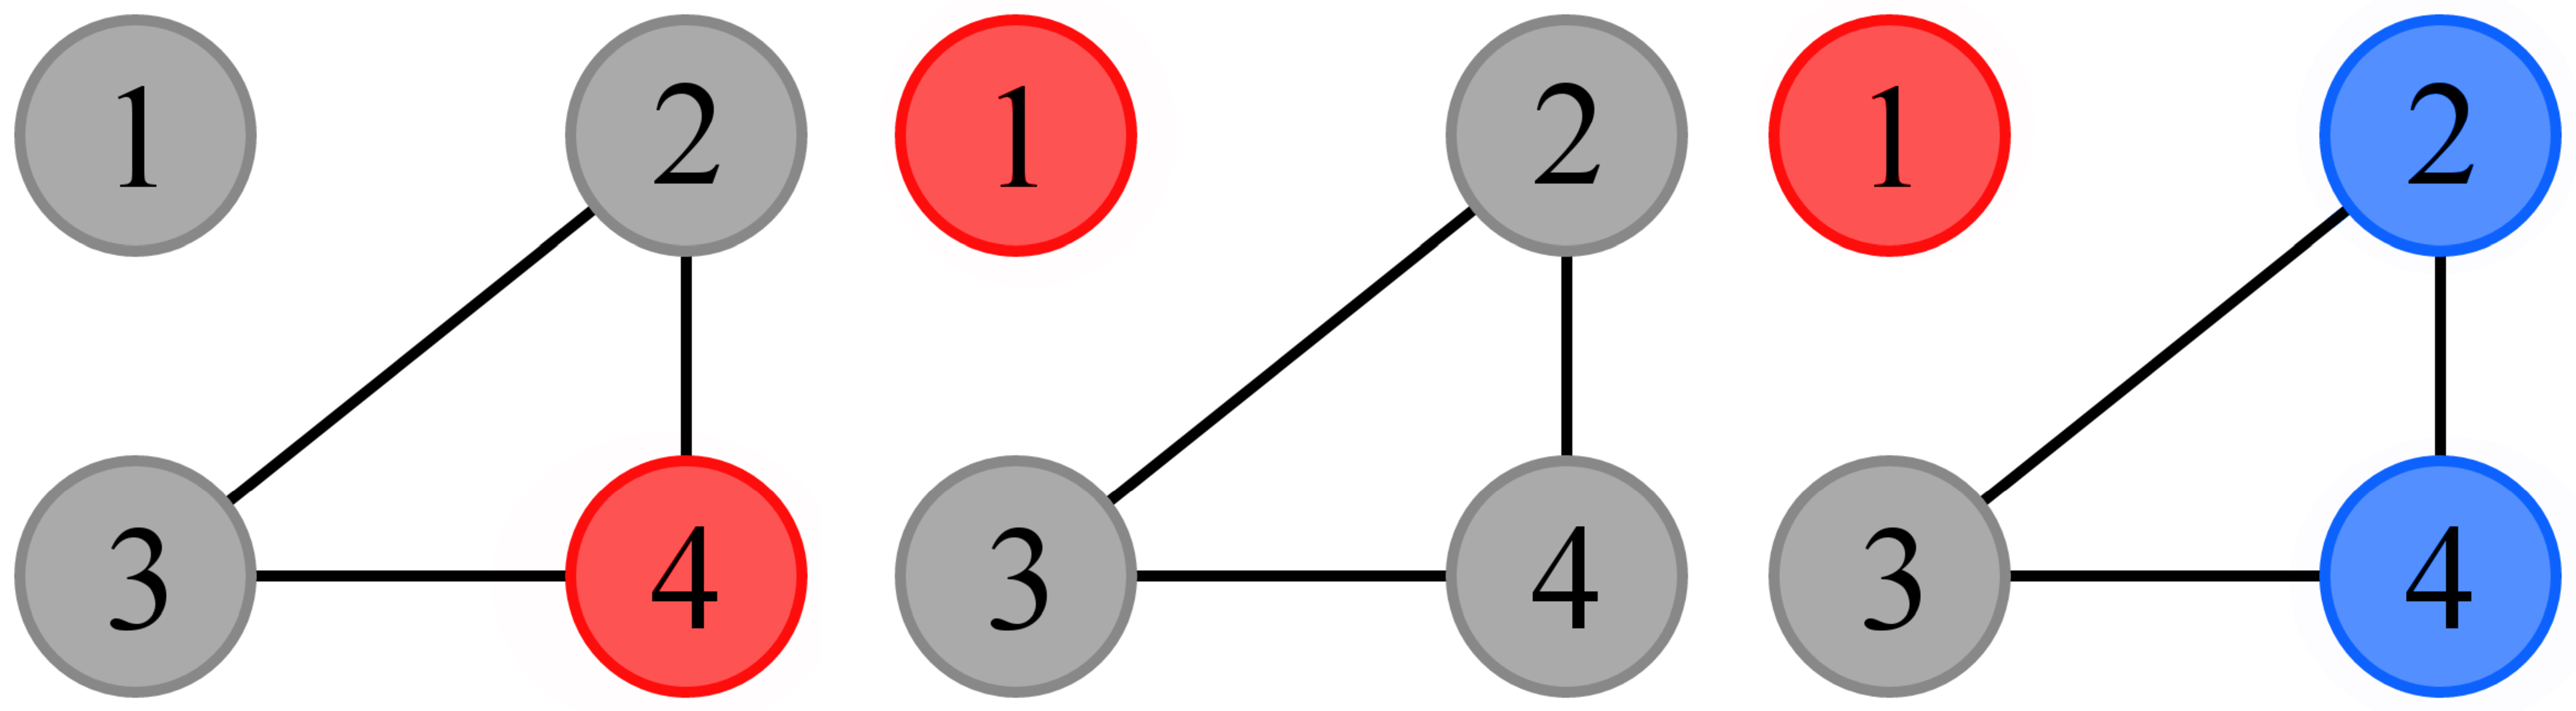
\includegraphics[width=10cm]{../figures/examples-1-incorrect.pdf}
    % \end{textblock*}
    %
    % \begin{textblock*}{\examplewidth}(0cm,5.2cm) % {block width} (coords)
    %   \centering
    %   Correct colorings
    % \end{textblock*}
    %
    % \begin{textblock*}{\examplewidth}(0cm,6cm) % {block width} (coords)
    %   \centering
    %   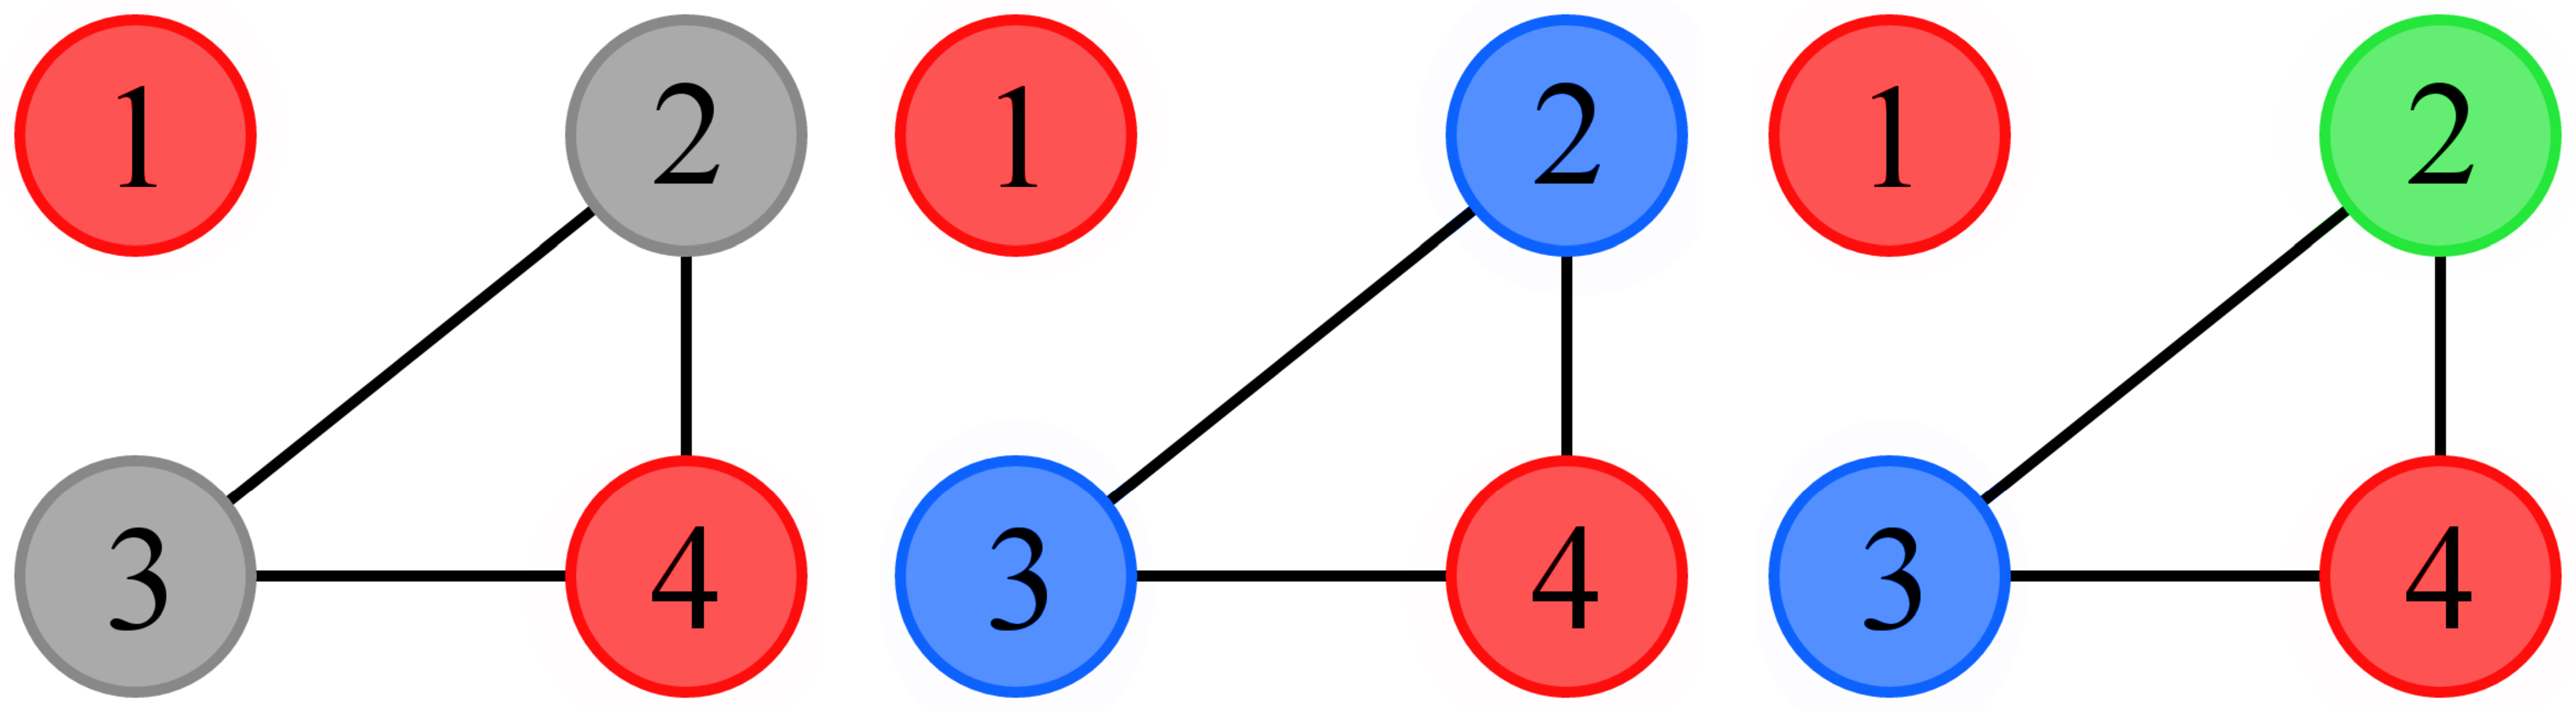
\includegraphics[width=10cm]{../figures/examples-1-correct.pdf}
    % \end{textblock*}

  \end{frame}

  \addtocontents{toc}{\protect\vspace{14pt}}

  \section{Applications}

  \subsection{Wireless Networks}

  \subsection{RFID Networks}

  \addtocontents{toc}{\newpage}


  \section{CF Coloring for General Graphs}

  \section{CF Coloring for Planar Graphs}

  \begin{frame}[standout]
    \centering
    {Thanks to Peter Dolan, Elena Machkasova,

    and Peh Ng for their advice and feedback.}
    \vfill
    \href{https://github.com/devshawn/senior-seminar}{github.com/devshawn/senior-seminar}
    \vfill
    \ccbyncsa{}
  \end{frame}

\end{document}
